\documentclass[10pt]{book}

\usepackage[utf8]{inputenc}
\usepackage[T1]{fontenc}
\usepackage[english]{babel}

\usepackage{array}
\usepackage{longtable}
\usepackage{adjustbox}
% Identificação
\newcommand{\thetitle}{Proof of concept on clustering using firmographics variables applied to a recommender system, a case study at Neoway}
\newcommand{\theauthor}{Matheus Frata}
\newcommand{\theadvisor}{André Carvalho Bittencourt}
\newcommand{\thecoadvisor}{Felipe Campos Penha}
\newcommand{\theplace}{Florianópolis}
\newcommand{\thedate}{2019}


% Paper geometry
\usepackage[a5paper]{geometry}
\geometry{tmargin=20mm, bmargin=15mm,
  lmargin=25mm, rmargin=15mm,
  % lmargin=20mm, rmargin=20mm, % Texto centralizado
  headheight=7mm, footskip=7mm}

% Graphics
\usepackage{graphicx}
\graphicspath{{fig/}}
\usepackage[font=small]{caption}
\usepackage[font=footnotesize]{subcaption}
\usepackage{color}
% Latin Modern font
\usepackage{lmodern}

% Hyperref configuration % Not necessary
\usepackage[hidelinks]{hyperref}
\hypersetup{pdftitle={\thetitle},
  pdfauthor={\theauthor}}

% Reformats section and subsection titles
\usepackage{sectsty}
\sectionfont{\sffamily\large}
\subsectionfont{\sffamily\normalsize}
\partfont{\sffamily\Huge}

% Fancy chapter
\usepackage[Sonny]{fncychap}

% Fancy header customization
\usepackage{fancyhdr}
\fancyhead{} % Clear all header fields
\fancyfoot{} % Clear all footer fields
\fancyhead[EL]{\sffamily\footnotesize{\thepage}}   % even, left
\fancyhead[ER]{\sffamily\footnotesize{\leftmark}}  % even, right
\fancyhead[OL]{\sffamily\footnotesize{\rightmark}} % odd, left
\fancyhead[OR]{\sffamily\footnotesize{\thepage}}   % odd, right
\pagestyle{fancy}

% Removes headers and footers for pages between chapters
\usepackage{emptypage}

% Line spacing
\usepackage{setspace}
\setstretch{1.1}
\renewcommand{\arraystretch}{1.25}

% Change numbered lists to lowercase roman numerals
\usepackage{enumerate}
\renewcommand{\labelenumi}{(\textit{\roman{enumi}})}
\newcounter{tmpc} % This is for resuming an 'enumerate' list

\newcommand{\cleardoublepageempty}{\clearpage
  {\pagestyle{empty}\cleardoublepage}
}

% incluir referencias bibliográficas no sumário
\usepackage[nottoc,notlot,notlof]{tocbibind} 
\usepackage{algorithm}
\usepackage[noend]{algpseudocode}
\usepackage{float}

%Package for colored tables
\usepackage[table,xcdraw]{xcolor}


\newcommand{\An}{A_{\text{n}}}
\newcommand{\Acn}{A_{c\text{n}}}

%\usepackage{amsmath,amssymb,amsthm}
\usepackage{bm}
\usepackage{thmtools}

\makeatletter
\def\blfootnote{\gdef\@thefnmark{}\@footnotetext}
\makeatother

% THEOREMS
\newtheorem{theorem}{Teorema}[chapter]
\newtheorem{lemma}[theorem]{Lema}
\newtheorem{corollary}[theorem]{Corolário}
\newtheorem{claim}[theorem]{Afirmação}
\newtheorem{fact}[theorem]{Fato}
\newtheorem{proposition}[theorem]{Proposição}
\newenvironment{example}[1][Exemplo. ]{\medskip\par\noindent\textsc{#1}}{\qed\par\medskip}
\newenvironment{definition}{\medskip\par\noindent\textsc{Definição.}}{\par\medskip}
\newenvironment{remark}{\medskip\par\noindent\textit{Observação:}}{\par\medskip}



%% Body
\begin{document}
  \begin{titlepage}
  \begin{center}
    
\includegraphics[width=2cm]{brasao-ufsc.pdf}
    % Brasão da UFSC
  \end{center}

  \begin{center}
    {\small FEDERAL UNIVERSITY OF SANTA CATARINA}\\
    {\small TECHNOLOGICAL CENTER}\\
    {\small ELECTRICAL AND ELETRONICS ENGINEERING DEPARTMENT}
  \end{center}

  \vfill

  \begin{center}
    \setstretch{1.75}
    {\LARGE \thetitle}
  \end{center}

  \vfill

  \begin{center}
  Undergraduate Thesis presented to the Federal University of Santa
  Catarina as a requisite for the bachelor degree of Electronics 
  Engineering.
  \end{center}

  \vfill

  \begin{center}
    {\large \theauthor}

    \medskip
    Advisor: \theadvisor\\
    %Co-advisor: \thecoadvisor
  \end{center}

  \vfill

  \begin{center}
    \theplace, \thedate.
  \end{center}
\end{titlepage}

\cleardoublepageempty

					 
  \pagenumbering{roman} 
  \begin{titlepage}
  \begin{center}
    {\large \MakeUppercase{\theauthor}}
  \end{center}

  \vfill

  \begin{center}
    \setstretch{1.5}
    {\Large \bfseries \MakeUppercase{\thetitle}}
  \end{center}
  \begin{flushright}
  	\begin{minipage}{0.5\textwidth}
     Undergraduate Thesis presented to the Federal University of Santa
     Catarina as a requisite for the bachelor degree of Electronics 
     Engineering.\ Advisor: \theadvisor. Co-advisor: \thecoadvisor
  	\end{minipage}
  \end{flushright}
  

  \vfill

  \begin{center}
    {\large \bfseries \MakeUppercase{\theplace} \par 2019}
  \end{center}
\end{titlepage}

  \thispagestyle{empty}
% Instructions: https://portal.bu.ufsc.br/servicos/ficha-de-identificacao-da-obra/
% Generation: http://ficha.bu.ufsc.br/

\mbox{}
\vfill

\begin{center}
    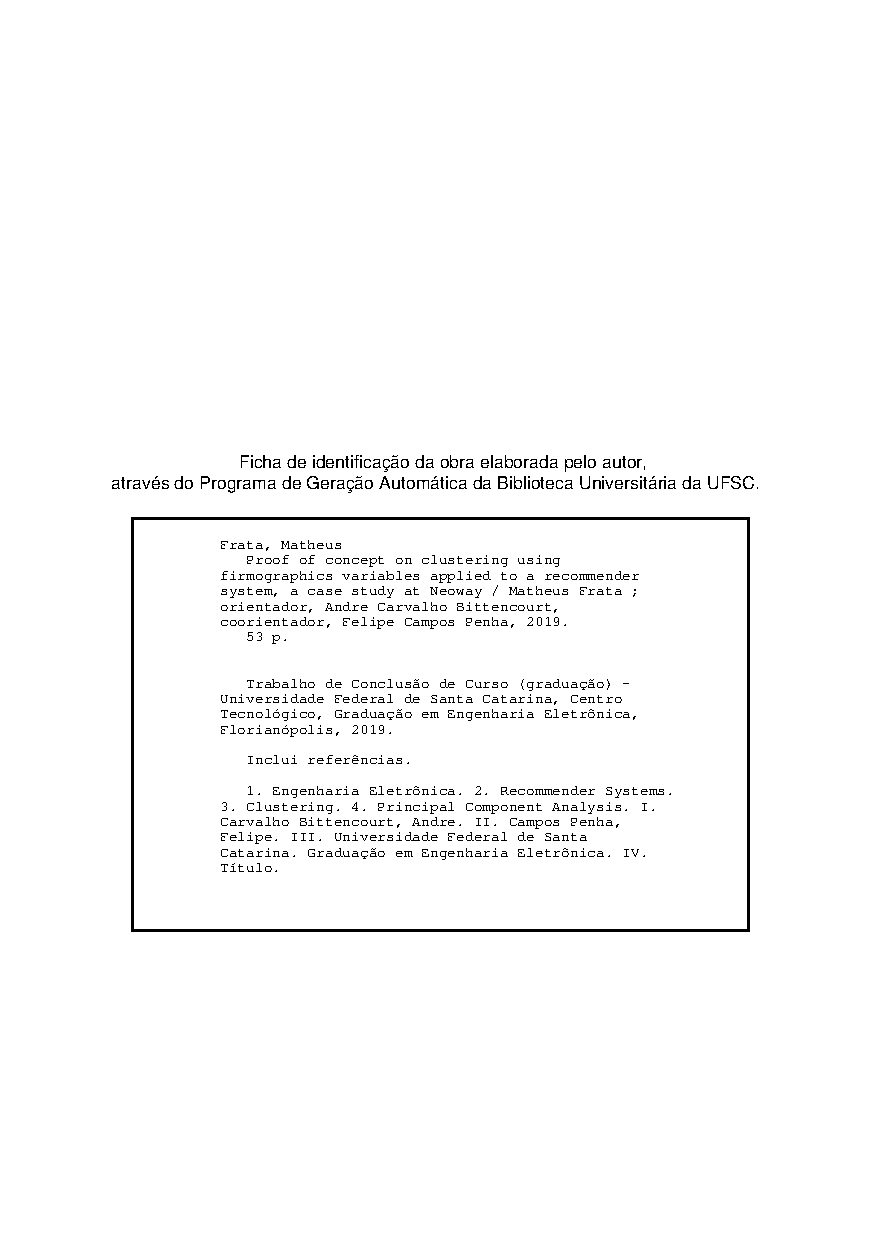
\includegraphics[width=\textwidth]{cartographics-a5.pdf}
\end{center}

\vfill
\mbox{}

\cleardoublepageempty

  \thispagestyle{empty}

\begin{center}
  \theauthor
\end{center}

\medskip
\begin{center}
  \textbf{\MakeUppercase{\thetitle}}
\end{center}

\medskip
\noindent {\small Este Trabalho de Conclusão de Curso foi julgado 
adequado para a obtenção do título de Bacharel em Engenharia Elétronica
e aprovado em sua forma final pelo Curso de Graduação em Engenharia 
Elétronica.}

% Versão pra impressão (sem assinaturas)

% Para melhor qualidade scanear (ou então após usar algum editor de imagens) cada assinatura separadamente, como exemplo a Figura assinatura01.png

\begin{center}
	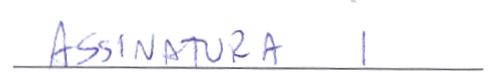
\includegraphics{assinatura01.png}\\
	\theadvisor, Ph.D.\\
	{\footnotesize Neoway Business Solutions}
\end{center}
\medskip
\textbf{Banca examinadora:}
\bigskip
\begin{center}
	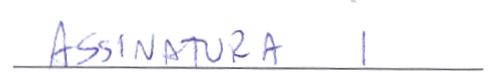
\includegraphics{assinatura01.png}\\
	Danilo Silva\\
	{\footnotesize Universidade Federal de Santa Catarina}
\end{center}
\bigskip
\begin{center}
	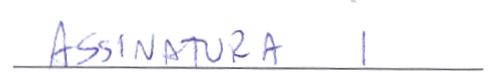
\includegraphics{assinatura01.png}\\
	Richard Demo Sousa\\
	{\footnotesize Universidade Federal de Santa Catarina}
\end{center}
\bigskip
\begin{center}
	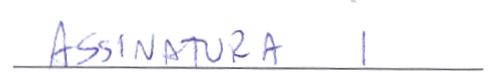
\includegraphics{assinatura01.png}\\
	Membro da Banca 3.\\
	{\footnotesize Universidade}
\end{center}
\medskip

\cleardoublepageempty

  \thispagestyle{empty}

\mbox{}
\vfill
\begin{flushright}
  \textit{Dedicatória}
\end{flushright}
\bigskip

\cleardoublepageempty

  \thispagestyle{plain}

\section*{Acknowledgments}

\indent First and foremost, I want to highlight the education from my parents, Adelar and Valdete. Their lessons and guidance enabled me to stand where I am today, and I cannot put in words how grateful I am for their support.

Secondly, I want to say "I love you" to the girl that I met way back when I still was in high school. She has been supporting me ever since. It has been 8 years of love, partnership and friendship. Thank you very much my Dear Caroline!

Thirdly, I want to give a shout out for all the folks that experienced UFSC life with me and still in contact: Lari, Zimpel, Griep, Ion, Karina, Roberto, Ruan, Claudio, Gui, Alevato, Elder, Eiterer. Also other folks that come and go: Giu, Penteado, Pedro Lemos, Kupas, Tortato. Deni you are going to deliver my certificate at my graduation!! (If you are reading this, and your name did not make it to this list, you should get in touch with me!!). Moreover, I want to thank the people from the institution: the faculty of EEL and other departments, the public employees of UFSC, and the labs that gave an opportunity to me: the Spacelab and the LCS.

Finally, I want to thank Neoway for the opportunity to develop this work. Specially the people at the Analytics Team! These people are the reason, for me, that makes Neoway a great place to work. Thank you very much for André, Penha, Igor, Breno, Mariana, Leandro, Vitor, Roger, Yuri, Leonardo, Felix, and Manoel. Also, a shout out for other teams (like the girls from GG and guys of SEC), and other employees that are not in the company anymore, but somehow had their contributions to my career!
% Hope didn't miss someone



\cleardoublepageempty

  \thispagestyle{plain}

\medskip

\begin{center}
  \textbf{RESUMO}
\end{center}



\bigskip

Este trabalho apresenta um método de.

\textbf{Palavras-chave:} Palavra1.Palavra2. Palavra3. 

\cleardoublepageempty

\thispagestyle{plain}

\begin{center}
	\textbf{ABSTRACT}
\end{center}

\bigskip

This work presents a method of.

\textbf{Keywords:} Word1. Word2. Word3.
  \chapter*{Acronyms}

% Because of a bug --- Force headers:
\fancyhead[ER]{\sffamily\footnotesize{\MakeUppercase{Acronyms}}}
\fancyhead[OL]{\sffamily\footnotesize{\MakeUppercase{Acronyms}}}

\begin{center}
  \begin{longtable}
    {>{\centering}m{0.15\textwidth} >{\small}m{0.75\textwidth}}
    \multicolumn{1}{c}{} & 
    \multicolumn{1}{l}{} \endhead
    RS      & Recommender System. \\
    PCA     & Principal Compoponent Analysis. \\
    AB      & bla bla bla bla. \\
    ABC     & bla bla bla bla. \\
    ABCD    & bla bla bla bla. \\
     \end{longtable}
\end{center}

  \setcounter{tocdepth}{2}

{\sffamily \listoffigures}
\cleardoublepageempty


{\sffamily \listoftables}
\cleardoublepageempty


{\sffamily \tableofcontents}
\cleardoublepageempty

  \label{pg:roman-count}
  \cleardoublepage

  \pagenumbering{arabic}
  \chapter{Introduction} 
\label{ch:introduction}

% Because of a bug --- Restore original headers:
\fancyhead[ER]{\sffamily\footnotesize{\leftmark}}
\fancyhead[OL]{\sffamily\footnotesize{\rightmark}}

Neoway Business Solution is a Big Data Analytics company with solutions to Sales \& Marketing and Risk \& Compliance that are suited to companies in a variety of business verticals and branches. One of its products is called On Target(OT), a lead recommendation system, based on scoring potential markets according to a given portfolio of clients. The OT will search for leads in a subset of the whole Brazilian's market space, which is composed by all active companies. The user can narrow down the search space based on a set of filters. The Figure \ref{fig:braz-comps-venn-diagram} shows a Venn diagram that illustrates the subsets of the On Target. The \underline{Portfolio} set is composed by the user's clients; The \underline{Market} is where the On Target will search for the leads, it can vary from a set defined by the filters to all the Brazilian active companies (except the user's clients).

\begin{figure}[!ht]
   \centering
   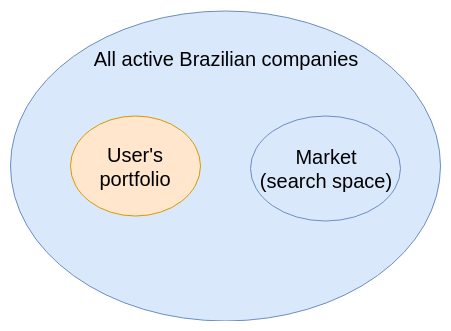
\includegraphics[width=9cm]{fig/ch1-brazil-comps-venn-diagram.png}
   \caption{Venn Diagram representing the sets involved in the recommender system.}
   \label{fig:braz-comps-venn-diagram}
\end{figure}

Recently, the OT was updated, and a benchmark was created to compare between different versions. Overall the new version showed an improvement in the accuracy performance and consistency of the recommendation. By analysing cases in the benchmark, we conjectured that the performance could be further improved in some cases if perhaps the user's portfolio had been pre-clustered before running the recommender system, leading to a more homogeneous and consistent scoring of the market. The last point can be understood through Figure \ref{fig:simi-dist} which shows the distribution of the recommender score in a benchmark case. The recommender system is trained with samples from the user's portfolio and market and its score allows for an interpretation of a similarity measure. The higher the score, going from $0$ to $1$, the more similar is a company to companies in the user portfolio, i.e. the more similar they are, and are thus better qualified to be converted to a lead or client.

\begin{figure}[!ht]
    \begin{subfigure}{\linewidth}
        \centering
        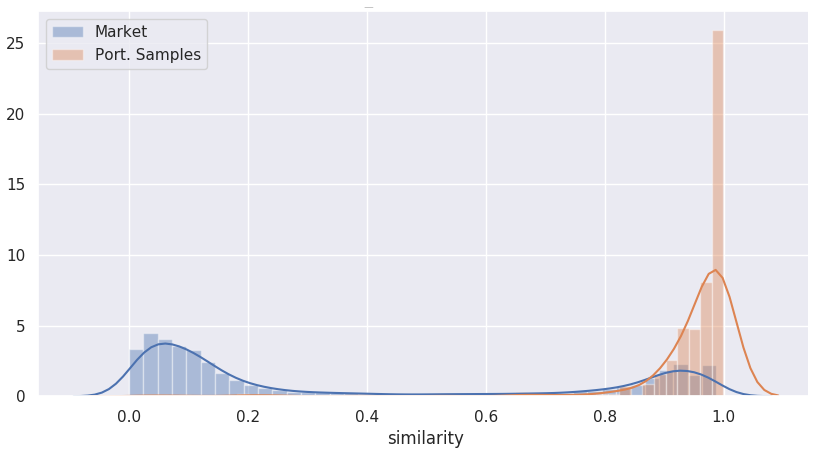
\includegraphics[width=10cm]{fig/ch1-simi-dist-expected.png}
        \caption{}
        \label{fig:simi-dist:expected}
    \end{subfigure}
    \begin{subfigure}{\linewidth}
        \centering
        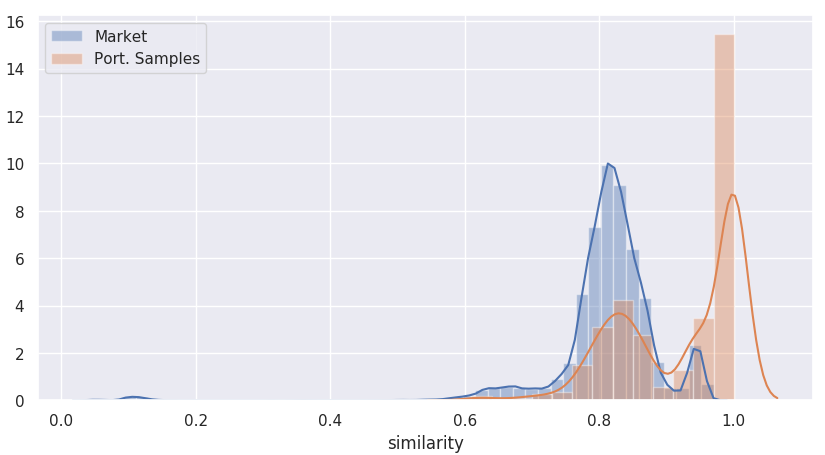
\includegraphics[width=10cm]{fig/ch1-simi-dist-to-investigate.png}
        \caption{}
        \label{fig:simi-dist:to-investigate}
    \end{subfigure}
    \caption{Similarity score from a case at the benchmark. (\subref{fig:simi-dist:expected}) shows a best case scenario one and (\subref{fig:simi-dist:to-investigate}) scenario to be investigated.}
    \label{fig:simi-dist}
\end{figure}

Similarity is how similar a company in the market is with the user's clients. The blue curve shows the recommender system is trained with samples from the user's portfolio and market and allows its score allows for an interpretation of a similarity measure. The higher the score, going from $0$ to $1$, the more similar is a company to companies in the user portfolio, i.e. the more similar they are, and are thus better qualified to be converted to a lead or client.\footnote{More about the similarity distribution plot will be explained on the chapter \ref{ch:methodology}.}
% OBS: "high density probabilities areas" = "bump"
\ref{fig:simi-dist:expected} is the best case scenario of a study, where all the portfolio's samples are close to similarity 1; The market has two high density probabilities areas: one close to similarity 0 and other close to similarity 1, in others words, some companies have no fit with the portfolio and others are alike the portfolio. The latter is the high quality leads to recommend to the user. \ref{fig:simi-dist:to-investigate} is an example of a study with a behavior may be improved. The portfolio's sample distribution has two concentrations of mass along the x-axis which can be interpreted that there were two types of customer's within the user's portfolio set. The aim of this thesis is to investigate whether this behavior can be improved by a pre-clustering strategy.

One hypothesis of the On Target's team is that in this study (and others alike) the client has a heterogeneous portfolio, \textbf{meaning that it can have two or more distinct profiles in it}. The algorithm tries to optimize for the mean profile of the whole portfolio which may not be the best approach.

This work is one of the several improvements that have been considered in the On Target Product Roadmap. It is a proof of concept which its objective is to analyze whether the overall performance of the high quality leads generation improves by clustering the portfolio before running the recommendation algorithm. 

In order to preserve interpretability, the clustering procedure will not include all available features. Only firmographics data will be used \cite{wikipedia_firmographics} which are data related to characteristics of a business, such as: company size, location, number of employees and others.


\section{Objectives}

\subsection{General Objectives}

The general objective of this work is to analyze whether the performance of the OnTarget improves by pre-clustering the portfolio with firmographics data before running the recommendation algorithm.

\subsection{Specific Objectives}

Specific objectives of this work are:

\begin{itemize}
    \item defining the pre-clustering strategy;
	\item defining the pre-clustering algorithm;
    \item defining the number of clusters for the benchmark cases;
    \item running OnTarget against the benchmark with the pre-clustering approach; and
    \item analyzing the distribution of similarity scores and performance metrics against the benchmark.
\end{itemize}


\section{Work outline}

This thesis is organized in the following manner: 

In the Chapter 2 some theoretical concepts are explained, so the reader can understand the what theory is behind this work. 

Next, in the Chapter 3, we introduce the terminology used by the OT's team and a basic view of how it works, later in the chapter, a discussion about the pre-clustering procedures and the conceived experiments.

In Chapter 4, is presented the results of these experiments alongside an extensive analysis in the metrics of several scenarios. 
 
Finally, in Chapter 5, a recap of this work is presented to the reader, with the takeaways. 
  \newcommand{\ASKA}{$\text{ASK}^0$}
\newcommand{\ASKS}{$\text{ASK}^*$}

\chapter{Literature Review}

In this chapter some basic concepts are presented to the reader to contextualize the work. First, it will be introduced the concept of recommender system (RS) and its importance in today's digital business strategies. Second, the metric used to evaluate the performance of the RS algorithm: lift. After that, a general discussion on clustering will be presented followed by one technique to visualize the clusters in a dataset: Principal Component Analysis.

\section{Recommender systems}

A RS is a software which its main purpose, as the name suggests, is to give suggestions \cite{ricci2011introduction} or recommendations to a user based on information about the user itself or the context of the items to recommend. They are classified as part of information filtering systems \cite{RecommendersystemWikipedia}. So, another way to interpret the recommendations is to think as the result of a filter applied on a search space, where only the most relevant information is given back to the user. It is important to emphasize that usually the search space on the RSs today are enormous. For example, there are more than 400 million products on Amazon US available \cite{amazon-number-of-products-2015}. Meaning that, in terms of time, it is unreasonable for a human to search one by one, analysing multiple attributes of millions of items at the same time. Hence, the importance of this type of system on the applications today.

\subsection{Types of Recommender Systems}

There are three main types: based on \textbf{collaborative filtering}, the ones on \textbf{content-based filtering}, and \textbf{hybrid}. 

The first one is \textbf{collaborative filtering}, where the recommendations come mainly from information generated by the user and its interaction with the items. For instance, one type of logic is the \textbf{user-based}, where a item is recommended to the user based on what other similar users like, more known as \textit{people like you, also like X}. Another logic is the \textbf{item-based} one, where the RS acts based on the similarity between items, also known as \textit{if you like X you may like X}. Figure \ref{fig:colab-filt-user-user} shows an example of user-based collaborative filtering, where the RS wants to predict what is the preference on headphones of user E. Based on users B and C (they voted similarly to E), we can see that, probably its a \textit{dislike}.

\begin{figure}[h]
   \centering
   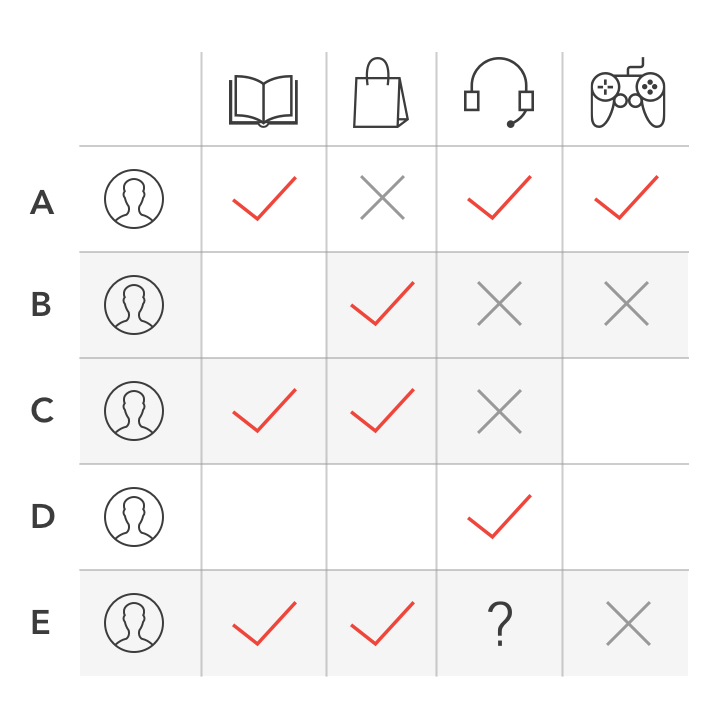
\includegraphics[width=6cm]{fig/ch2-colab-filt-user-user.jpg}
   \caption{User-based logic on collaborative filtering. Source: \cite{delawareai}}
   \label{fig:colab-filt-user-user}
\end{figure}

The second one is \textbf{content-based filtering}, where the recommendations are based on the features of the items and more importantly: an \textbf{user profile}. The system needs an input from the user, be it interactively like in a sequential manner or historical data, or in batch where the user gives a lot information about itself at once. Having the profile, the RS can cross this information with the features of the items to look for items that are similar to the user's profile. It can remember the item-based logic from collaborative filtering, but here we have added the information of the user. One example that illustrate content-based, is an article reader service. Imagine when one signs up to the service, it will ask a lot of question to the new user: "What type of articles do you prefer: Sports, Politics, Health?", "What kind of Sports do you like: Soccer, Volleyball, Baseball...?". These questions build up a profile of the new user and it will be refined as the users utilizes the service. Therefore, if our hypothetical new user answers "Sports" and "Soccer" to the previous questions, the article service will start recommending articles of soccer. But if this new user only thumbs up Brazilian Soccer articles, the RS will learn that and narrow down the recommendations to Brazilian soccer.

Finally, there is the \textbf{hybrid} type, where the Recommendation System is based on a mixture of both previous types. Combining them can improve the recommendations and at the same time deal with their constraints. Collaborative filtering has the problem of \textbf{cold start}, whenever a new item or user is added, it has no attributes. So it will take some time until its attributes are filled up. This problem leads to another one which is the \textbf{sparsity} on the matrix of attributes. Meaning that, there are a lot of missing values. Content-based filtering can supply this data to the RS. And combining with the accuracy of collaborative filtering the system can achieve very personalized recommendations.


\subsection{Benefits to business}

The RSs are present on a myriad of online services today, bringing great value to them. Streaming platforms of music and videos have RSs on their business to increase user retention and engagement such as: $75\%$ of what people watch on Netflix come from recommendations \cite{HowretailerscankeepupwithconsumersMcKinsey} or that $70\%$ of people's time spent on YouTube comes from the recommendation of "the Algorithm" \cite{CES2018YouTubesAIrecommendationsdrive70percentofviewingCNET}. Social medias and reading platforms apply these same concepts on their "feed" for those same reasons, user retention and engagement. E-commerce, on the other hand, want to increase their revenue by recommending similar products, or products that the "same type of customer purchased" when a potential customer is navigating on their online shop. Amazon is a great example of this: $35\%$ of the purchases on their online shopping come from recommendations \cite{HowretailerscankeepupwithconsumersMcKinsey}. There is even the use of RSs on online dating services \cite{brozovsky2007recommender}, where the RS improve the experience of the user in the search of potential partner while at the same time increasing the monetization of the service.

Netflix is one of the companies that are references on this type of system. They have a variety of algorithms on their RS. And due to the high user base, they can test their results using A/B testing and feedback from the users \cite{gomez2016netflix}. IN 2006 they launched a competition, called the Netflix Prize, where the objective was to improve the accuracy of the recommendations by $10\%$. The winner would win one million dollars. There were more than 2.000 teams and more than 40.000 submissions on their platform. The Netflix prize was an important event to the RSs in general because it increased the awareness of this technology, and its importance to business, worldwide. 

\subsection{Evaluation}
\label{ch:evaluation}

There are several ways to evaluate the performance of a recommender system: normalized Discounted Cumulative Gain (nDCG) \cite{jarvelin2002cumulated}, Precision \cite{Precision-rs-metric}, Recall \cite{cremonesi2010performance} when "looking" to the RS with a ranking perspective; Mean Absolute Error (MAE) \cite{breese1998empirical} and Root Mean Squared Error (RMSE) \cite{bennett2007netflix} when "looking" to the RS with a rating perspective; A/B testing when you have a high client base that guarantee statistical relevance and others \cite{parra2013recommender}. To evaluate the Neoway's recommender system we chose the Lift.

Lift is a ratio between probabilities. The probability of selecting one of the target population after the RS sorting versus the random  chance (before the RS sorting). The lift, is usually expressed in terms of quantiles. \cite{LiftAnalysisADataScientistsSecretWeapon}.

Suppose your market set is given $\mathcal M$ with size $|\mathcal M |\!=\!N$ and let the subset $\mathcal L \supset \mathcal M $, with $|\mathcal L|\!=\!n$, represent all companies within the market that would lead to a conversion. The set $\mathcal L$ is of course unknown and the problem is to chose a strategy that recommends companies in $\mathcal M$ such that it is also belongs to $\mathcal L$. The probability for a random strategy is uniform across the population and is given by $n/N$. Suppose now that to each company $X_i$ you associated a score $S_i$ and ordered the companies from the highest to lowest score, i.e. $S_i>S_{i-1}$ for all $i$ and started picking from $S_N$ to $S_1$. For any $k$, the lift is how much better this strategy is up to $k$ relative to the random strategy, i.e.
\begin{equation}
    \mathrm{lift}_k = \frac{P(X_{i:k\leq i\leq N}\in \mathcal L)}{n/N}.
\end{equation}


To illustrate further, let us use an example of a box with colored balls. Imagine that there is a rectangular box where its height and depth allows only a single ball to fit, but its width allows up to 100 balls. There are two types of balls: the \textbf{red} ones that represent our \textbf{target population} and the blue ones. 90 of the 100 balls are blue and the remaining 10 are red. Moreover, this box is divided into sectors where each sector is a decile, meaning that there are 10 sectors, each one with 10 balls. The sectors, also, have a priority, they from left to right. Figure \ref{fig:rec-box} shows hows this box looks like.

\begin{figure}[h]
   \centering
   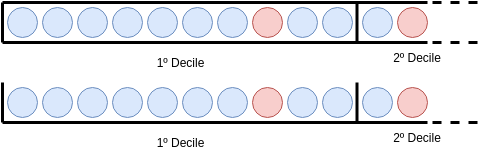
\includegraphics[width=\linewidth]{fig/ch2-rec-box.png}
   \caption{Rectangular box. Upper view (above), Front view (below). }
   \label{fig:rec-box}
\end{figure}

Without seeing inside the box, the probability of retrieving a red ball is 10 out of 100, or \textbf{$10\%$}. This is our \textbf{random chance} and it is the same probability for each decile. Now lets consider that someone reordered the balls (representing the RS), trying to place the red ones on first deciles. The Figure \ref{fig:rec-box-ordering} shows the box before and after the reordering.

\begin{figure}[h]
   \centering
   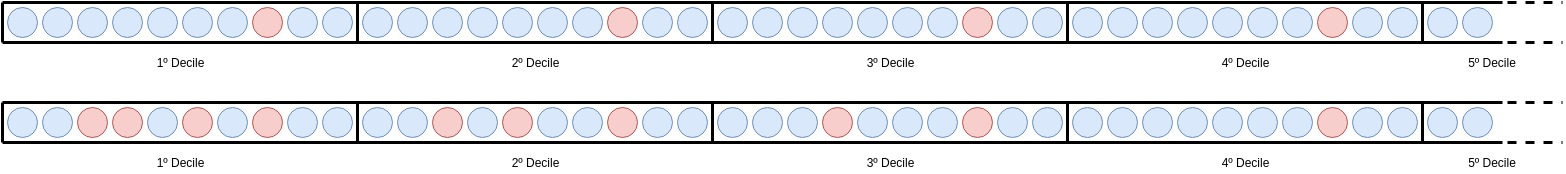
\includegraphics[width=\linewidth]{fig/ch2-rec-box-ordering.jpg}
   \caption{Reordering of the balls. Before (above) and after (below).}
   \label{fig:rec-box-ordering}
\end{figure}

After the reordering, we recalculate the probabilities of retrieving a red ball for each decile. We can see on Figure \ref{fig:rec-box-ordering}, that there are 4 red balls on the first decile, 3 on the second, 2 on the third and 1 on the fourth. With this information we have the following probabilities, respectively: 40\%, 30\%, 20\%, 10\% and 0\% to the remaining deciles. Now the lift for the deciles can be calculated, for the first one is:
\begin{equation}
	lift_{1\textsuperscript{o} decile} = \frac{0.4}{0.1} = 4
\end{equation}

Using the same approach, we calculate the lift for the others deciles, respectively: 3, 2, 1, and 0 to the remaining ones. Figure \ref{fig:lift-plot} shows a plot of the values of the lift for each decile.

\begin{figure}[h]
   \centering
   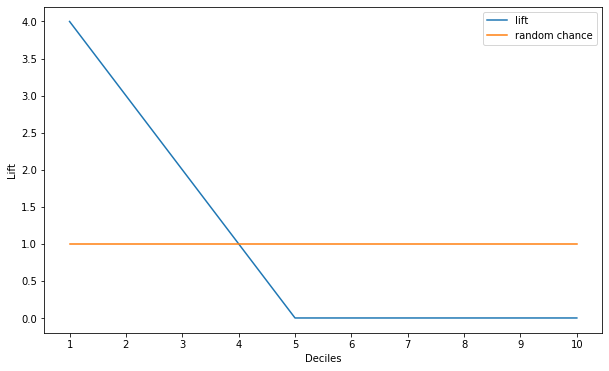
\includegraphics[width=9cm]{fig/ch2-lift-plot.png}
   \caption{Lift plot for the reordered box with the random chance.}
   \label{fig:lift-plot}
\end{figure}

We can see that it is more likely to pick a red ball on the firsts sectors of our box (deciles) than in the last ones. Actually, there is a zero probability to get a red ball after the fourth decile, since all balls are to the its left. And this is the expected behavior, since in an information retrieval system (IRS), we want all the relevant information on the top (in our case: on the left). Hence, only the first $N$-quantiles (in our case: $N = 10$) are considered and the rest is discarded. The designer of the system should decide how many quantiles are included and it also depends on how much information is retrieved and how much can be processed by the user.

With this example, another way to interpret the lift is: how many times better than the random chance it is to get relevant information in the first $N$-quantiles ordered by an IRS.

\section{Clustering}

% what % why
Cluster Analysis is an unsupervised learning technique where its objective is to find a finite and discrete set of "hidden" structure in a dataset \cite{xu2008clustering}. These structures or patterns can help better understand data or serve as a preprocessing step for algorithms. Clustering can also be a way to represent large amounts of information which is equivalent to compressing data. 

% where
This technique is applied in several areas \cite{sabine2001cluster}. For instance, in Engineering and Computer Science, clustering is used in speech recognition, information compression, noise removal. In biology, the applications are: genetics, taxonomy, microbiology and others; It is also used in Astronomy and Geography on classification of galaxies, planets for the former and classification of regions, areas, vegetation and land for the latter.

% how
There are various approaches used to cluster a dataset \cite{wikipedia_cluster_analysis}. The Connectivity-based method looks for the closeness of two objects, meaning that it forms the clusters based on their relative distance which can be computed in different ways like the complete (maximum distances) or simple (minimum distance) linkage methods. The Hierarchical Clustering is an example of algorithm that uses this approach; On Centroid-based clustering the data is represent by a vector of centroids - we can think of them like center of mass - one for each cluster. The KMeans algorithm (and its variations), uses this approach. The Distribution-based approach focus on the statistics of the dataset. It groups together objects that have similar distributions. The algorithms to exemplify this are the Gaussian Mixture and its Bayesian variation. Another one is the Density-based clustering where the data is grouped on the high density areas. Points that are to far away are considered outliers and do not go to any cluster. Common algorithms are the DBSCAN and the OPTICS.


% caveat
There is no single best algorithm on cluster analysis \cite{james2013introduction}. All of these mentioned, have pros and cons and are fit to different kind of problems. Some are suited to find the number of clusters but at the same time do not scale with a high volume of data (Hierarchical) \cite{franti2006fast}, others are fast and simple but they have to know the number clusters in advance (KMeans). Hence, it is important to test different algorithms and their parameters to see if the analysis perform on a given problem.

\section{Principal Component Analysis}

% what
Principal Component Analysis, or PCA for short, is an orthogonal linear transformation \cite{wikipedia_pca} where you "break down" a dataset - that can have correlation between the dimensions - into an independent set of variables called \textbf{Principal Components}. These components maintain the original data variance, or in practical terms, the amount of information. They are sorted in a descending fashion, where the first principal component (PC$_{1}$) has the most variance and PC$_{N}$, has the least variance. $N$ goes up to the number of the smallest dimension (rows or columns), the minimum between these two. 

%how
To understand how the PCA works in an intuitive way, Figure \ref{fig:pca-steps} illustrates the steps of the PCA algorithm on a dataset with two variables.

\begin{figure}[h]
   \centering
   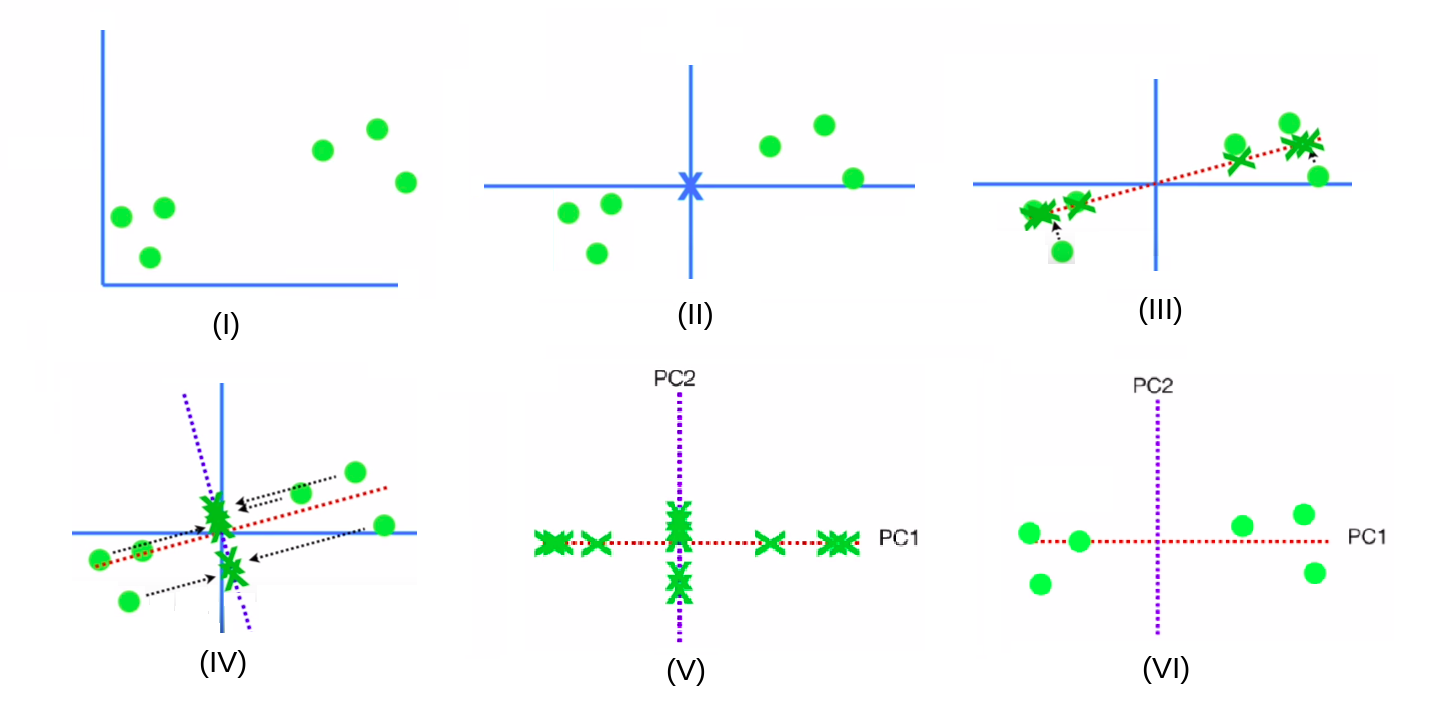
\includegraphics[width=\linewidth]{fig/ch2-pca-steps.png}
   \caption{Steps of PCA for two variables. Source: Adapted from \cite{pcastepsyoutube}.}
   \label{fig:pca-steps}
\end{figure}

From the original data: (I) we calculate the mean point (center of mass), by getting the means of the x-axis and y-axis. Then we make this point our new origin (II). After that, a line that goes through the origin is fitted on the data on the direction of the highest variance (III). This direction is obtained by maximizing the sum of squared distances from the origin of each point's projection on the line(represented by the green Xs). The best fitted line is the Principal Component 1 (PC$_{1}$). From a projection orthogonal to PC1, the process repeats from (I) to find PC$_{2}$ which is the second-highest-variance direction. However, since this example there are only two variables, there is only one possible direction (IV). With PC$_{1}$ and PC$_{2}$ calculated, when can make them our new axis (V) and use the points' projections (V) to find where they go on the PCA plot (VI). For a dataset with more variables the process is the same: data is centered; each PC$_{N}$ line should point to the direction of $N$-highest variance and every PC$_{N+1}$ must be orthogonal to PC$_{N}$.

%why and where
PCA can be applied to any numerical dataset \cite{wold1987principal} (first it must be transformed or scaled). It can be a useful tool to analyse any multi-variable data. One use of this technique is the \textbf{PCA plot} which consists on getting the first two or three principal components (PCs) and plotting the transformed data. Since most of the variance (information) is on the first PCs, we can use them to look for patterns on the dataset with 2-D or 3-D plots. One of the patterns that can be found are clusters \cite{ding2004k}. 

Another use of PCA is \textbf{dimensionality reduction}. Imagine that there is a dataset with more than 200 variables. Due to the curse of dimensionality \cite{Bellman:2010:DP:1893145} or even computing power a reduction on the number features is needed. If by applying PCA on this dataset we get, for instance, $99\%$ of the variance on the first 20 PCs, the remaining PCs can be discarded. In practice, we are getting a $90\%$ data reduction with only $1\%$ of the information lost.






  \chapter{Methodology}
\label{ch:methodology}

In this chapter it will be explained how the cluster analysis and the experiments were conducted. The first part of the chapter is dedicated to define some concepts related to the On Target product: the OT itself and its benchmark project. The second part is about the cluster analysis. And the third one is about the experiments.

\section{About the Product}

Before getting to the clustering and experiment procedures, it is important to define some concepts about the OT product. A high level explanation of the OT and how its benchmark was built will be described in this first part of the chapter.

\subsection{On Target}

The On Target is one of the Neoway's products of the vertical of B2B Sales and Marketing. Neoway's customers, which are business, use the OT to look for other business that have the potential to become their customer. It achieves that through content-based recommendations, strictly speaking, the OT searches for potential costumers for Neoway's clients based on their clients. To create the recommendations OT need the following inputs:
\begin{itemize}
    \item the \textbf{Portfolio}, which is the list of companies that are customers of the OT user. It can range from a few dozens to dozens of thousands companies;
    \item the \textbf{Market}, which is the list of companies where the OT will search for the leads. It can range from dozens to tens of millions companies; and
    \item the \textbf{Features}, which is a data set with the characteristics of the companies.
\end{itemize}
And it outputs the sorted \underline{Market} based on a score called \textbf{Similarity}. Figure \ref{fig:ot-blocks} illustrates a block diagram of the OT.

\begin{figure}[h]
   \centering
   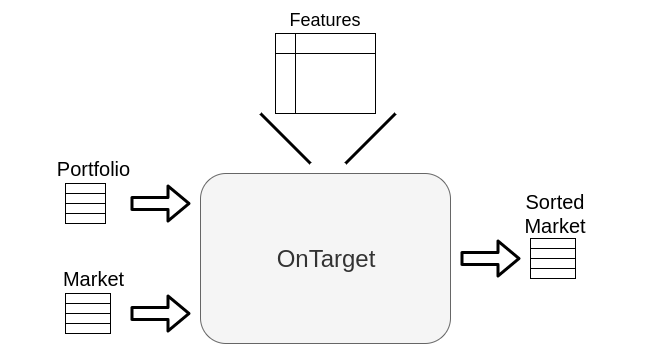
\includegraphics[width=\linewidth]{fig/ch3-ot-blocks.png}
   \caption{Block Diagram of the On Target. Source: Author}
   \label{fig:ot-blocks}
\end{figure}

\subsection{Benchmark}

As mentioned on the chapter \ref{ch:introduction}, the recommender system was update and one of the ways to assure that the modifications had a positive impact on the algorithm was to develop a benchmark. The Benchmark is a project that compares different versions of the OT, by running these versions on almost thirty different business scenarios. They can be: one retail customer with a huge portfolio and huge market size; or a bank with a small portfolio and medium market size; or even a service provider with small portfolio and small market size. A run of the OT for one of this scenarios is called a \textbf{Study}. An \textbf{Experiment} is the run of all of these scenarios for new versions of the OT comparing to the current one that it is running on production. Every modification on the algorithm generates a new experiment. For instance, if the number of features is increased, an experiment (or more) is generated. If a parameter of the algorithm is changed, a new experiment is generated.

The Benchmark does some minor modification on the OT pipeline. It removes a random sample of companies from the portfolio (it can be 10\%, 30\% or 50\%) and it places them on the market. The idea is to use this sample as holdout set \cite{kohavi2001}, which is a separated part of the data used for test. For the OT these companies are in the market, without "knowing" that they came from the portfolio, therefore it is expected that the companies in the holdout set have a high score (similarity) on the output. Figure \ref{fig:ot-benchmark-blocks} shows these modifications on the OT.

\begin{figure}[h]
   \centering
   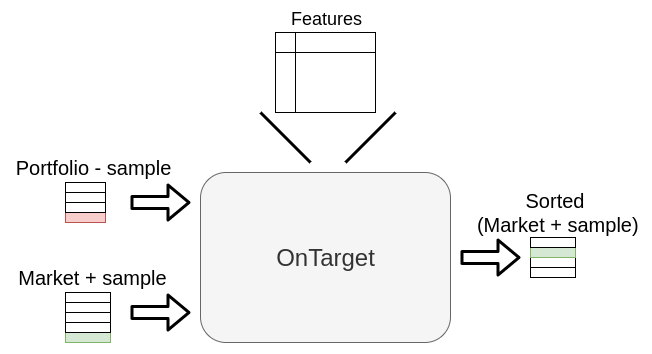
\includegraphics[width=\linewidth]{fig/ch3-ot-benchmark-blocks.png}
   \caption{Modifications on the OT done by the Benchmark. Source: Author}
   \label{fig:ot-benchmark-blocks}
\end{figure}

These changes on the pipeline are to generate the metrics to evaluate the experiments in two ways. The first one, is the performance with the \textbf{lift}, usually only the first decile. The second one is consistency, with the \textbf{similarity distribution} plot. On the former, the holdout set is used to calculate the probabilities after the sorting of the OT - similar to the red balls analogy discussed on \ref{ch:evaluation}. The latter, plots the distribution of the scores assigned to the market and to the holdout set. As seen on the Introduction chapter of this work, Figure \ref{fig:simi-dist-expected-real} shows an example of this plot, where the orange are the holdout set and the blue curve is the market.

\section{Clustering}

In this seconds part of the chapter it will be explained how the clusters analysis were conducted. It will be explained how and what are the clustering strategies and clusters pairing. Also, a discussion about definition of number of clusters and the choice of the cluster algorithm.

\subsection{Clustering strategy and pairing}

% names for the cluster strategies
\newcommand{\nameClusterStrategyA}{TrainOnPort}
\newcommand{\nameClusterStrategyB}{TrainOnAll}
% names for the cluster pairing
\newcommand{\nameClusterPairingA}{PairWithItsCluster}
\newcommand{\nameClusterPairingB}{PairWithAllMarket}


The first thing to tackle was the definition of the clustering strategy and pairing. The \underline{clustering strategy} dictates how the clustering algorithm will be applied on the data, and the \underline{cluster pairing}, determines how the clusters from the portfolio will be paired with the clusters from the market.

There are two possible clustering strategies: \textit{training the cluster algorithm on the portfolio and applying it on the market} which will be called \textbf{\nameClusterStrategyA{}}, and \textit{training and applying on all the data} which will be called \textbf{\nameClusterStrategyB{}}. Let us take the example of the KMeans algorithm using these two strategies applied on a fake study dataset, which is illustrated on Figure \ref{fig:cluster-strategy}. Assuming that all sub plots are on the same scale, in (I) we see the portfolio clustered with its two centroids, on (II) we can see the KMeans "predicting"\footnote{this is a fairly common name for the inference step of an algorithm in scikit-learn implementation} the clusters of all data with the centroids learned on (I). This is the \nameClusterStrategyA{}. The \nameClusterStrategyB{} is represented on (III) where the KMeans trains and predicts on all data. We can see that the centroids are on different positions, as a result some companies are allocated on a different cluster relative to (II). 

\begin{figure}[h]
   \centering
   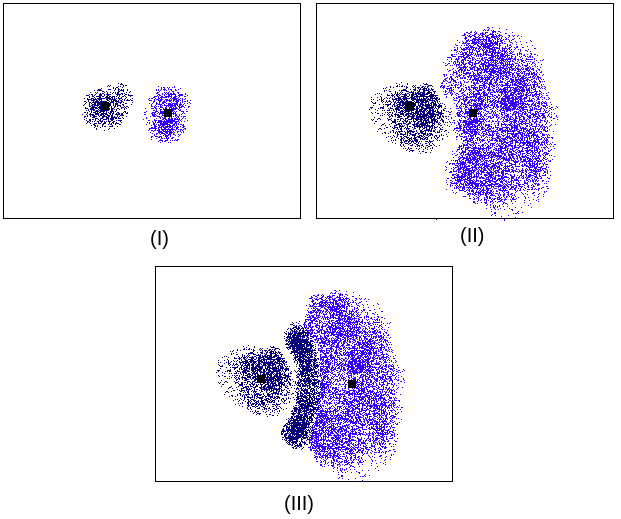
\includegraphics[width=9cm]{fig/ch3-cluster-strategy.png}
   \caption{Fake study data set that shows how both clustering strategies work. Source: Author}
   \label{fig:cluster-strategy}
\end{figure}

For the pairing there are also two possible ways: \textit{each cluster on the portfolio will be matched with its cluster on the market} (let us call it \textbf{\nameClusterPairingA{}}), and \textit{each cluster on the portfolio will run with the whole market} (let us call it \textbf{\nameClusterPairingB{}}). For instance, if we have a study that have three clusters on the portfolio with 50 companies each, and 150 companies on each cluster on the market, in \nameClusterPairingA{} the OT will run three times with a portfolio size of 50 and market size of 150; for \nameClusterPairingB{} the OT will run three times with a portfolio size of 50 and a market size of 450 (whole market for each cluster). Figure \ref{fig:cluster-pairing} shows a block diagram of this scenario.

\begin{figure}[h]
   \centering
   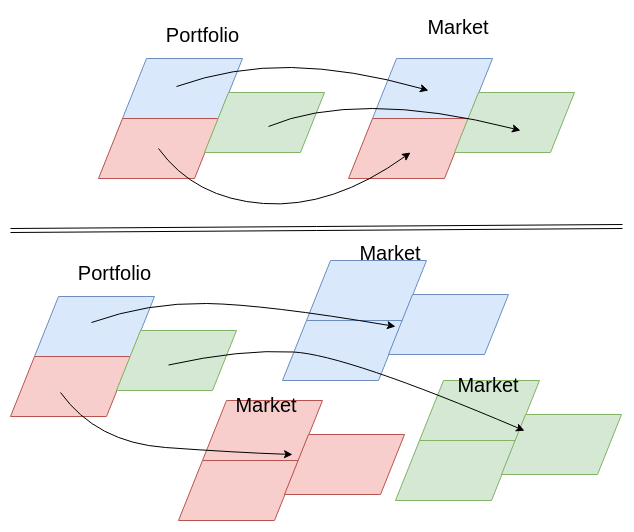
\includegraphics[width=7cm]{fig/ch3-cluster-pairing.png}
   \caption{Illustration of the cluster pairing. On the top is the \nameClusterPairingA{} and on the bottom the \nameClusterPairingB{}. Source: Author}
   \label{fig:cluster-pairing}
\end{figure}

Through a business view, it makes more sense to adopt the \textbf{\nameClusterStrategyA{}} since we are interested on the recommendations based on the user profile, in other words, the user's portfolio, regardless of the market data. 

On cluster pairing II the market is replicated for each cluster, leading each company to be scored N times (N being the number of clusters). Hence, there could be cases where one company has a high score in a cluster while, at the same time, have a low score in other one. To not deal with these cases the \textbf{\nameClusterPairingA{}} was chosen for this work.

\subsection{Number of clusters}

The second aspect of the cluster analysis was the number of clusters for each study, since most of the cluster algorithms need this information upfront. Even though, there are some research on evaluating the number of clusters automatically \cite{yu2014automatic}, there are no production-ready solutions. There are, however, methods like Elbow method and Silhouette \cite{kodinariya2013review} that help with the determination of the number of clusters, but they are not reliable 100\% of the time, meaning that it would be difficult to automate. Considering that the objective is to analyse the impact of the clustering on the RS and not the cluster analysis itself and that there are only up to thirty studies, it was decided to set the number of the clusters \textbf{manually}.

To visualize the clusters on the studies, it is necessary to plot the data. But OT uses too many variables on production to analyse all of it at once. Hence, it was applied PCA transformation on the studies and used the first two principal components to plot the transformed data and to see the patterns in it. 

Before applying the PCA, a preprocessing step was needed. Categorical features were converted to numeric using One Hot Encoding and all features were scaled using the Z-score Normalization\footnote{all of the data transformations functions used on this theses are from the Scikit-learn Python library \cite{scikit-learn}}.

Figure \ref{fig:pca-plot} shows the results of the PCA plot for some studies using all features that OT uses on production environment (top), and PCA plot using only firmographics features for the sames studies (bottom). Each study is a column, where the first row is the plot of the PCA for the portfolio data, the second row the PCA plot for the market data, and the third row is for both, using different colors to distinguish portfolio from market (blue is the market and orange the portfolio).

We can see that it is much more difficult to visualise the clusters on the all-features PCA plot. There are some examples where you see a clear boundary on the data, but if wee look to the firmographics plot these boundaries are much more defined. Moreover, if you take to account the business perspective, it makes sense to group the companies by their firmographics. For example, a study with one clusters with big companies from the state of São Paulo and the other one with small companies from the state of Santa Catarina.

Using the firmographics PCA plot, each study was assigned with a number of clusters manually. For instance, on Figure \ref{fig:pca-plot}, from left to right, the number of clusters in the portfolio assigned are, respectively: 3, 3, 3, 2, 4, 3, 2, 2.  

\begin{figure}[h]
   \centering
   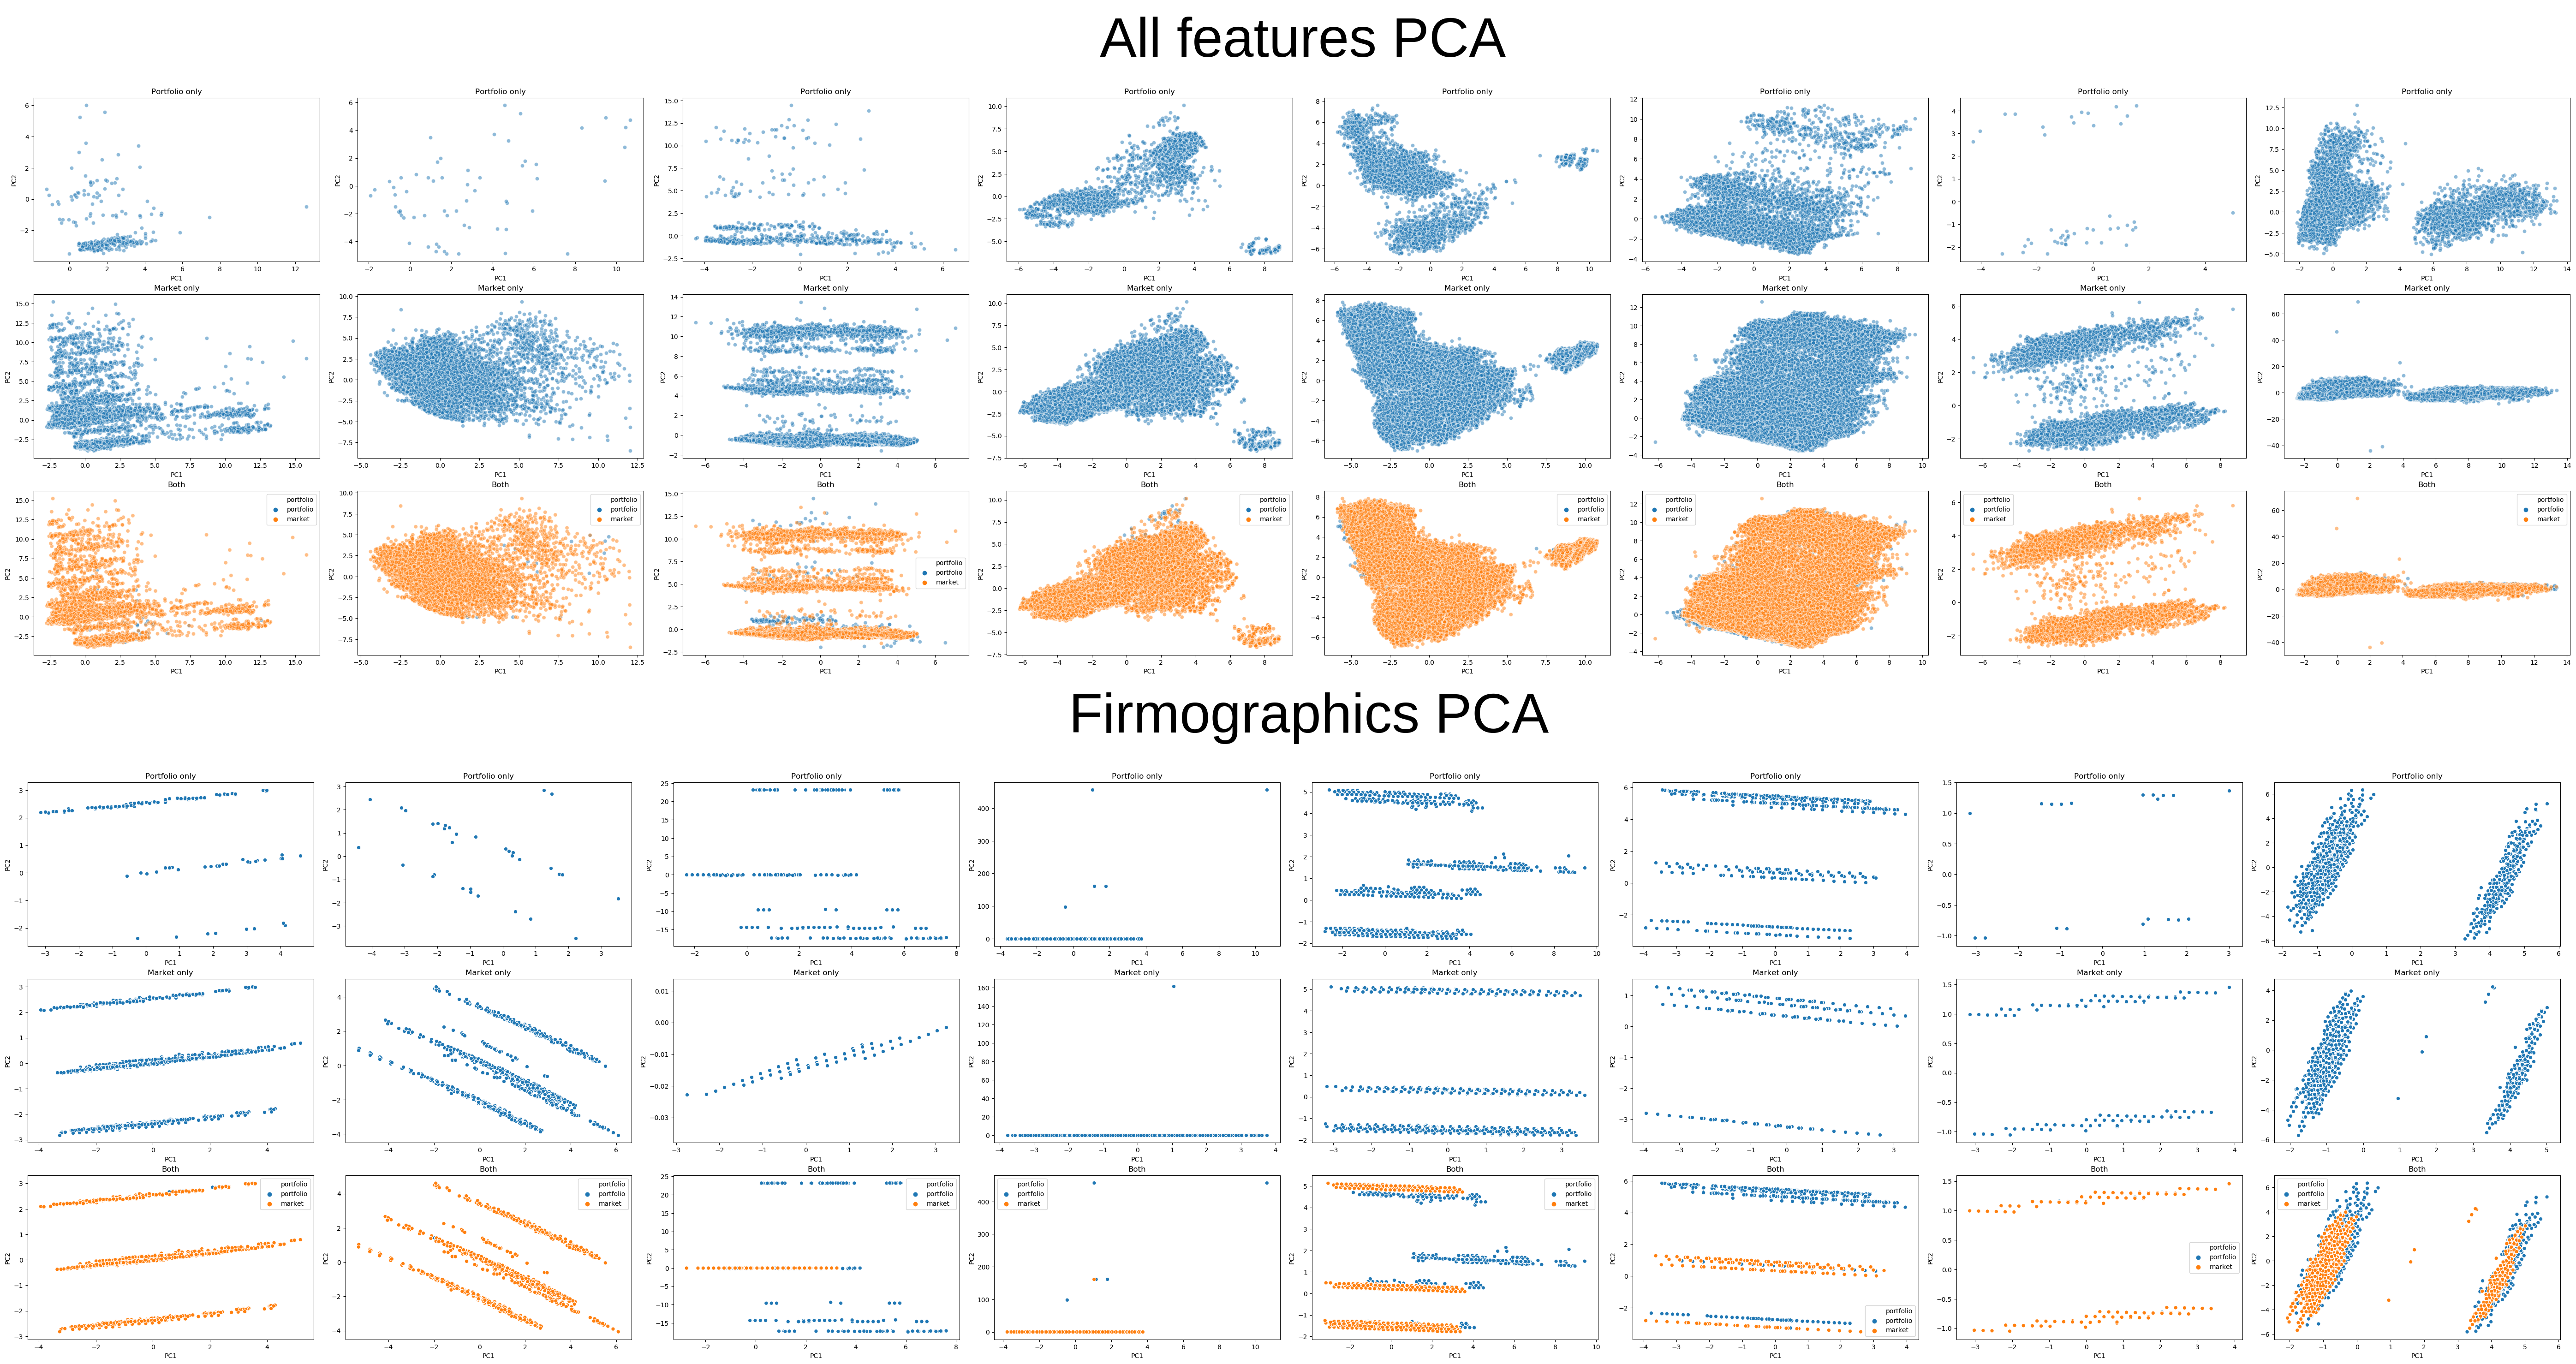
\includegraphics[width=\linewidth]{fig/ch3-pca-plot.png}
   \caption{PCA plot for the studies. On the top there is the the one using all features and on the bottom, only using firmographics features. Source: Author}
   \label{fig:pca-plot}
\end{figure}

\subsection{Cluster algorithm}
\label{ch:cluster-algorithm}

The last aspect of the cluster analysis was the choice of the algorithm. From the firmographics two principal components data, six clusters algorithms were applied on all the studies: \underline{KMeans}, \underline{Gaussian Mixture}, \underline{Bayesian Gaussian Mixture}, \underline{Agglomerative Clustering}, \underline{Spectral Clustering}, \underline{DBSCAN}\footnote{all of these implementations came from the scikit-learn python library \cite{scikit-learn}}. All of them were computed with default parameters and the same seed.

The last three did not run on some studies that have a market size in an order of magnitude of dozen of thousands companies, due to memory error\footnote{all the algorithms were running on a machine with 250 GB of RAM}. Because of their high memory complexity \cite{franti2006fast}, \cite{ester1996density}, \cite{yan2009fast}, they were discarded.

The studies were also clustered \underline{manually} in order to be used as a benchmark for the algorithms. "Manually" in a sense that the boundaries among the clusters were defined without an algorithm. Since, most of the PCA plots present a regression characteristic, these boundaries were lines equations. Figure \ref{fig:clustering-studies} shows the results for some of the studies using "Manual Clustering", KMeans, Gaussian Mixture (GMM) and Bayesian Gaussian Mixture (BayesianGM).

As we can see the algorithms did not get the shape of the data in some of the studies. The Bayesian and GMM had better results relative to the KMeans. But they did not assigned the clusters as expected, for instance, on the third and sixth row of Figure \ref{fig:clustering-studies}. Due to these reasons and the same argument explained on the number of clusters discussion - we are interested on the results on the RS and not in the cluster analysis itself - it was decided by the team to start to the experiments using the "Manual Clustering".

\begin{figure}[H]
   \centering
   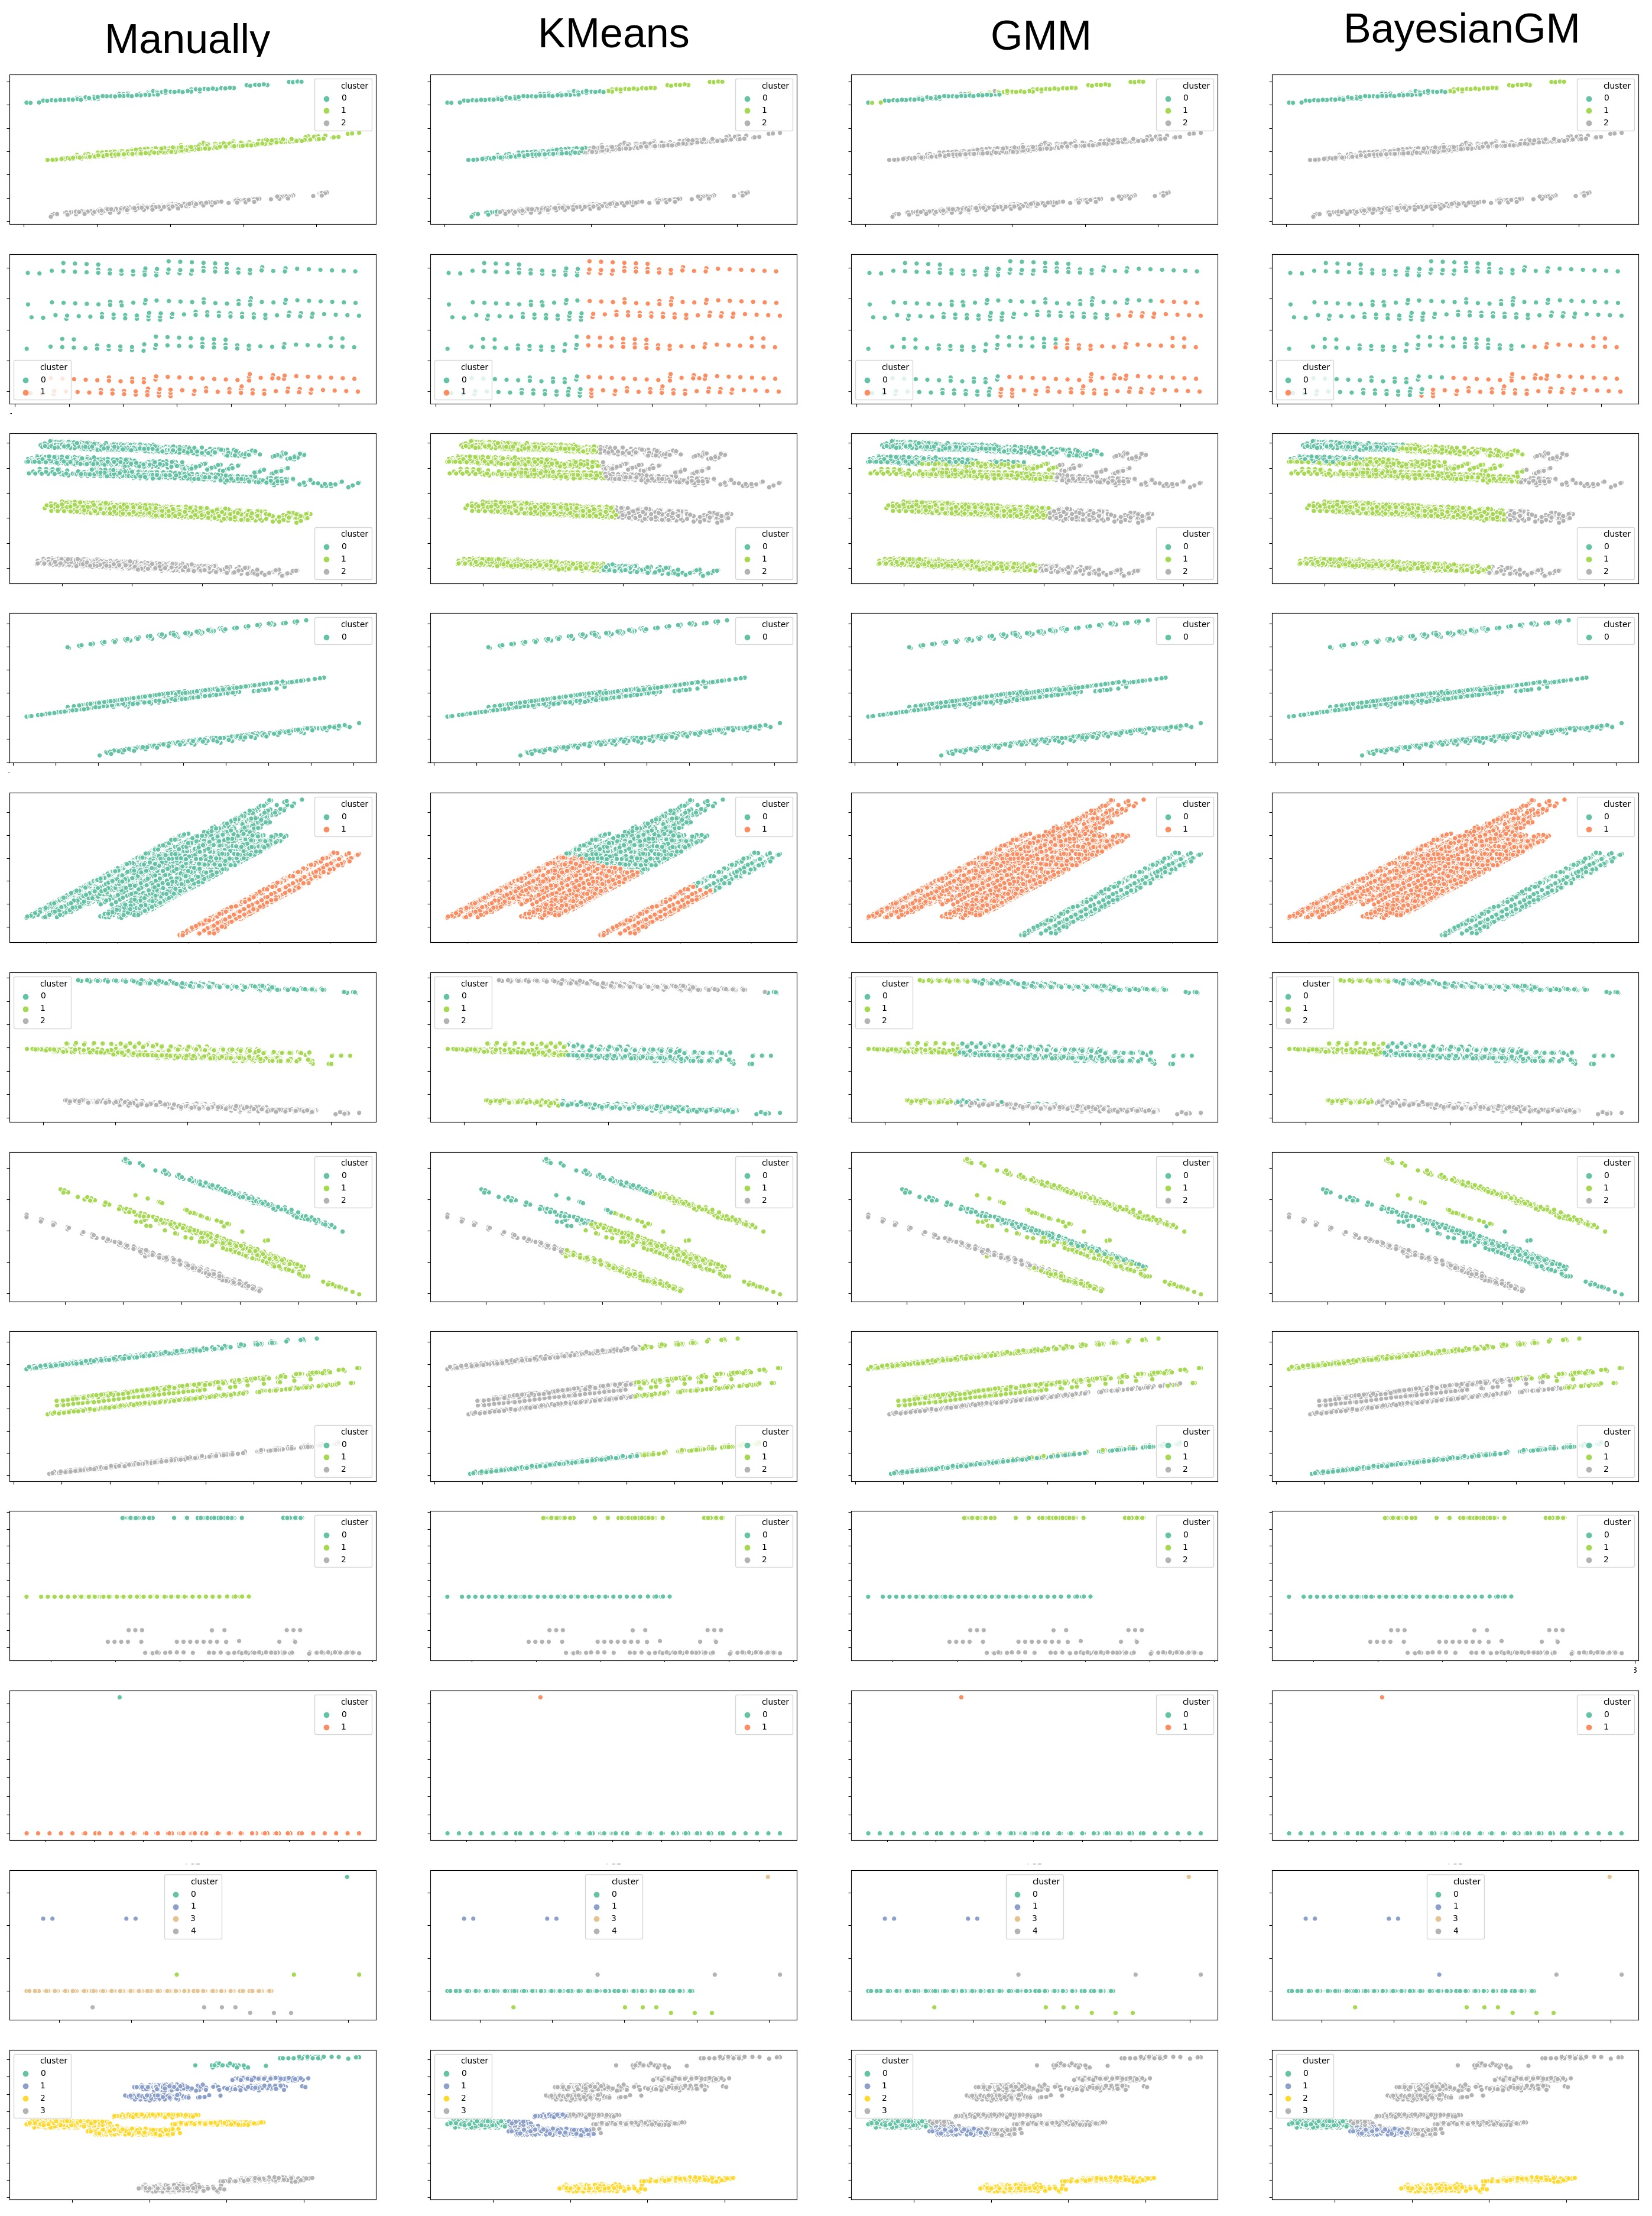
\includegraphics[width=\linewidth]{fig/ch3-clustering-studies.png}
   \caption{Results of the clustering on the first two principal components of some studies. Source: Author}
   \label{fig:clustering-studies}
\end{figure}

\section{Experiments}

% names for the experiments
\newcommand{\nameExperimentI}{OneRunEachCluster}
\newcommand{\nameExperimentII}{ClusterAsFeatures}


In this last part of the chapter, it will be discussed about the experiments that were developed to test the clustering in the OT. After the analysis of the clusters, it was formulated two experiments: \textbf{\nameExperimentI{}} and \textbf{\nameExperimentII{}}.

\subsection{One run for each cluster}
\label{ch:experiment-i}

The experiment \nameExperimentI{} consists on using the clustering strategy \nameClusterStrategyA{} and cluster pairing \nameClusterPairingA{}. A cluster in a portfolio will be matched with its pair on the market, and each cluster, on a study, will generated a run of the OT. After the runs, all of the outputs will be joined into a single one. So, for the user, the interface still the same. But, internally, OT will split the study in N\footnote{N is the number of clusters} smaller studies and then will aggregate the outputs. These modifications can be better understood when looking to the diagram on Figure \ref{fig:one-run-each-cluster}. 

\begin{figure}[h]
   \centering
   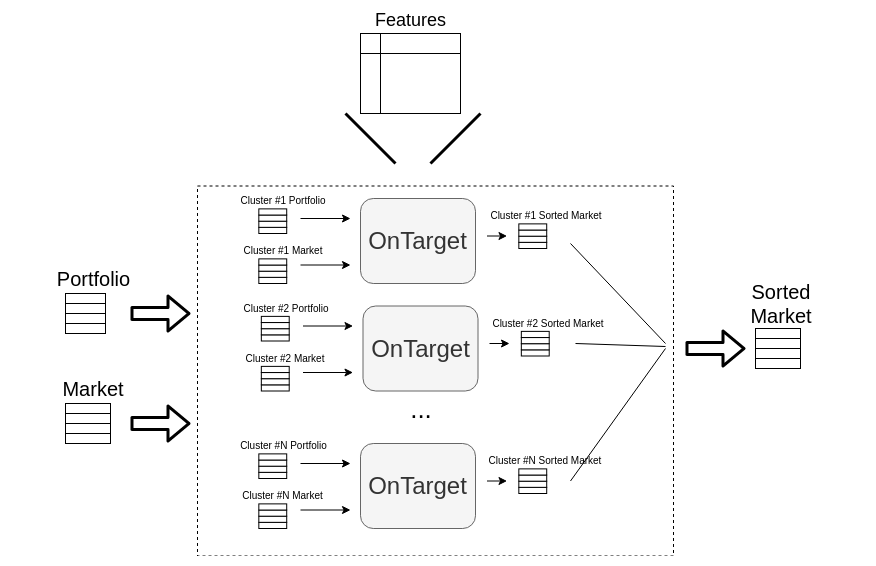
\includegraphics[width=\linewidth]{fig/ch3-one-run-each-cluster.png}
   \caption{Modifications on the OT for the experiment \nameExperimentI{}. Source: Author}
   \label{fig:one-run-each-cluster}
\end{figure}

To clarify more this idea of the Experiment \nameExperimentI{}, let us take the example of Figure \ref{fig:cluster-strategy}. Since there are two clusters, OT will match the dark blue cluster on the portfolio with its pair on the market, generating one run. Another run will be generated by using the same analogy for the light blue cluster. Then the OT will aggregated both outputs and return as only one sorted market.

Another important modification made on the OT pipeline due to the \nameExperimentI{} was the definition of a \textbf{minimum size to a study}. There could be cases where, in a portfolio, a cluster has a small number of companies that is not enough for the RS algorithm to create the score. A cluster (sub-run on the OT) must have at minimum:
\begin{itemize}
    \item \textbf{5} companies in the \textbf{portfolio};
    \item \textbf{2} companies in the \textbf{holdout sample}\footnote{in the experiment \nameExperimentI{}, the holdout set was sampled after the clustering}; and
    \item \textbf{10} companies in the \textbf{market};
\end{itemize}
If one of these is not satisfied, the data is discarded. For example, a study with a portfolio size of 40 and market of 40000, with 3 clusters and the following number of companies in the portfolio/holdout/market: \textbf{Cluster I: 3/1/4000}, \textbf{Cluster II: 20/4/30000}, \textbf{Cluster III: 9/3/6000}. The Cluster I run would be discarded, losing 10\% of the overall study market. Still, there are 36000 companies to search for leads, so it is not a significant loss. Moreover, creating a strategy to allocate these sub-studies' companies that are discarded in other clusters would be cumbersome and it would not be worth it since it is a small percentage of the overall study. Therefore, the discard approach was chosen due to its simplicity.

\subsection{Clusters as features}

The second experiment consists in using the information of the clusters as an extra column in the features table used by the OT. It will not use any of the cluster pairing strategies (it uses the clustering strategy I, though). The experiment \nameExperimentII{} is much more simple than \nameExperimentI{}: there is no split on the study; it is not necessary an aggregation of the output; and it is not needed to define a minimum number to a study to run. The information of the clusters is joined with the features table that feed the RS algorithm. Figure \ref{fig:clusters-as-features} shows its simple modification.

\begin{figure}[H]
   \centering
   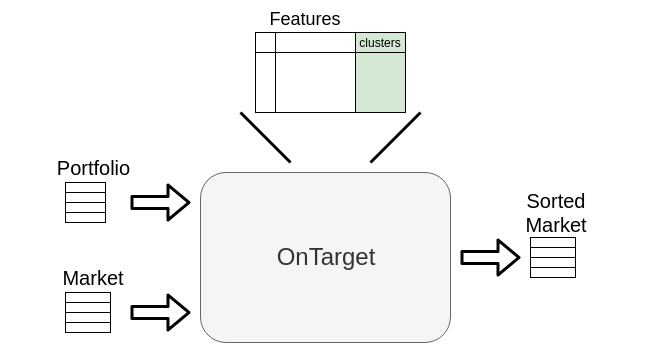
\includegraphics[width=\linewidth]{fig/ch3-clusters-as-features.png}
   \caption{Modifications on the OT for the experiment \nameExperimentII{}. Source: Author}
   \label{fig:clusters-as-features}
\end{figure}
  \chapter{Experimental results}

In this chapter we will present the results of the experiments \nameExperimentI{} and \nameExperimentII{}, along with a discussion of the impact on the lift and similarity distributions of these experiments relative to the OT without the clustering.

\section{Experiment \fullNameExperimentI{}}

As seen on \ref{ch:experiment-i} this experiment was the one that creates sub-runs of the OT for each cluster in the portfolio. Also, it had to be created some heuristics to deal with clusters that did not have enough data to run. Using the "manual clustering", as discussed on \ref{ch:cluster-algorithm} the summary of the lift gain (how much the lift on the first decile increased or decreased relative to the OT without clustering) is presented on Table \ref{table:lift_gain_exp-i}. Figure \ref{fig:lift-hist-plot-exp-i} shows another perspective for this data through a histogram, excluding the outliers studies.

The cells are colored to better understand the gains. The dark colors (green and red) represent a considerable positive or negative gain (more than 5\%), the light colors a slight positive or negative gain (less than 5\%). The white, represent that the lift did not change. Finally, the orange ones are the outliers which were defined using the interquartile range rule \cite{upton1996understanding}. 

\begin{table}[!ht]
\centering
\begin{adjustbox}{max width=7cm}
\begin{tabular}{|c|c|c|c|}
\hline
\textbf{Study} & \textbf{Lift Gain (\%)}        & \textbf{Study} & \textbf{Lift Gain (\%)}        \\ \hline
1              & \cellcolor[HTML]{ff514d}-12,09 & 15             & \cellcolor[HTML]{ff514d}-13,26 \\ \hline
2              & \cellcolor[HTML]{009901}16,67  & \textbf{16}    & \cellcolor[HTML]{ff514d}-20,00 \\ \hline
3              & \cellcolor[HTML]{00c901}0,89   & \textbf{17}    & \cellcolor[HTML]{ffccc9}-4,28  \\ \hline
4              & 0,00                           & 18             & \cellcolor[HTML]{ff514d}-13,06 \\ \hline
5              & \cellcolor[HTML]{ffccc9}-0,14  & 19             & \cellcolor[HTML]{ff514d}-15,42 \\ \hline
6              & \cellcolor[HTML]{ff514d}-17,28 & 20             & \cellcolor[HTML]{00c901}0,57   \\ \hline
7              & \cellcolor[HTML]{ff514d}-12,44 & \textbf{21}    & \cellcolor[HTML]{ff514d}-33,95 \\ \hline
\textbf{8}     & \cellcolor[HTML]{ffccc9}-5,17  & 22             & 0,00                           \\ \hline
\textbf{9}     & \cellcolor[HTML]{ff514d}-27,78 & 23             & \cellcolor[HTML]{ff514d}-28,16 \\ \hline
\textbf{10}    & \cellcolor[HTML]{009901}6,25   & 24             & \cellcolor[HTML]{ffce93}200,01 \\ \hline
11             & \cellcolor[HTML]{ff514d}-17,75 & \textbf{25}    & \cellcolor[HTML]{ff514d}-12,77 \\ \hline
12             & \cellcolor[HTML]{ffccc9}-1,01  & 26             & \cellcolor[HTML]{ff514d}-29,35 \\ \hline
13             & \cellcolor[HTML]{ff514d}-6,93  & 27             & \cellcolor[HTML]{ffccc9}-0,08  \\ \hline
14             & \cellcolor[HTML]{ffccc9}-1,16  &                &                                \\ \hline
\end{tabular}
\end{adjustbox}
\caption{Summary of the first-decile lift gains for Experiment \nameExperimentI}
\label{table:lift_gain_exp-i}
\end{table}

\begin{figure}[!ht]
   \centering
   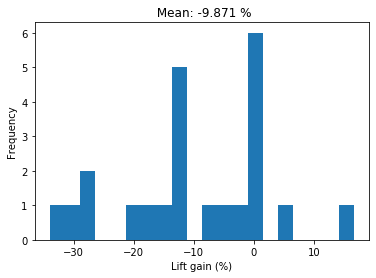
\includegraphics[width=8cm]{fig/ch4-lift-hist-plot-exp-i.png}
   \caption{Histogram plot of the studies' lift gain for experiment \nameExperimentI{}.}
   \label{fig:lift-hist-plot-exp-i}
\end{figure}

There are also some studies that are bolded. They represent the studies that brought up the hypothesis of this work, as discussed at the Introduction, they had two or more high density areas on the similarity distribution plot, meaning that, they can have more than one profile in their portfolio.

We can see that only five studies had positive impact on the lift, and one of them is an outlier. The majority of the studies had a negative impact, six of them were sightly negative and fourteen worsened the lift considerably. It is important to notice that two studies did not present any changes on the lift with the clustering. The overall mean lift gain for \nameExperimentI{} is $-9.871 \%$.


\section{Experiment \fullNameExperimentII{}}

Now for the second experiment, which was the simple use of the clustering information as another feature. Using the same color scheme as Table \ref{table:lift_gain_exp-i}, Table \ref{table:lift_gain_exp-ii} shows the summary of the lift gains for the experiment \nameExperimentII{}. Figure \ref{fig:lift-hist-plot-exp-ii} this data in a histogram (without outliers studies).

\begin{table}[!ht]
\centering
\begin{adjustbox}{max width=7cm}
\begin{tabular}{|c|c|c|c|}
\hline
\textbf{Study} & \textbf{Lift Gain (\%)}        & \textbf{Study} & \textbf{Lift Gain (\%)}        \\ \hline
1              & \cellcolor[HTML]{00c901}4,40   & 15             & \cellcolor[HTML]{00c901}0,46   \\ \hline
2              & \cellcolor[HTML]{ff514d}-8,33  & \textbf{16}    & \cellcolor[HTML]{ff514d}-6,58  \\ \hline
3              & \cellcolor[HTML]{009901}23,65  & \textbf{17}    & \cellcolor[HTML]{ffce93}-46,08 \\ \hline
4              & 0,00                           & 18             & \cellcolor[HTML]{ffccc9}-1,87  \\ \hline
5              & \cellcolor[HTML]{00c901}1,49   & 19             & \cellcolor[HTML]{00c901}3,58   \\ \hline
6              & \cellcolor[HTML]{ffce93}-28,33 & 20             & \cellcolor[HTML]{ff514d}-11,28 \\ \hline
7              & \cellcolor[HTML]{009901}12,50  & \textbf{21}    & \cellcolor[HTML]{ffccc9}-2,64  \\ \hline
\textbf{8}     & \cellcolor[HTML]{009901}16,84  & 22             & \cellcolor[HTML]{00c901}1,23   \\ \hline
\textbf{9}     & \cellcolor[HTML]{009901}12,80  & 23             & \cellcolor[HTML]{ffccc9}-0,14  \\ \hline
\textbf{10}    & \cellcolor[HTML]{009901}18,59  & 24             & \cellcolor[HTML]{ffce93}300,02 \\ \hline
11             & \cellcolor[HTML]{ff514d}-7,84  & \textbf{25}    & \cellcolor[HTML]{00c901}4,90   \\ \hline
12             & \cellcolor[HTML]{ffccc9}-0,15  & 26             & \cellcolor[HTML]{ffccc9}-0,77  \\ \hline
13             & \cellcolor[HTML]{00c901}0,68   & 27             & \cellcolor[HTML]{00c901}1,21   \\ \hline
14             & \cellcolor[HTML]{009901}7,30   &                &                                \\ \hline
\end{tabular}
\end{adjustbox}
\caption{Summary of the first-decile lift gains for Experiment \nameExperimentII}
\label{table:lift_gain_exp-ii}
\end{table}

We can see that, differently from \nameExperimentI{}, the majority of the studies had positive gain (16 studies, to be exactly). Only four studies were considerably worse on the lift gain and five sightly worse, a total of nine studies. Only one study did not present any change to the lift and, this time, four were outliers (two positives and two negatives). The mean lift gain for \nameExperimentII{} is $2.016 \%$.

\begin{figure}[!ht]
   \centering
   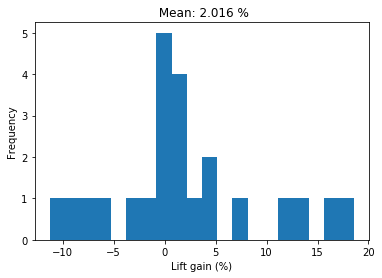
\includegraphics[width=8cm]{fig/ch4-lift-hist-plot-exp-ii.png}
   \caption{Histogram plot of the studies' lift gain for experiment \nameExperimentII{}.}
   \label{fig:lift-hist-plot-exp-ii}
\end{figure}

\section{Similarity distributions}
\label{ch:simi-distis}

Now let us look at some of the similarity distributions plots for both experiments. These plots will have three curves: the market similarity in green, the holdout set in orange, and the portfolio in blue. Each topic of this section will address a group represented by the colors in the lift gain summary tables. 

\subsection{Studies with no change to the lift}

In both experiments there were studies that did not lead to any change to the lift. Study 4 appeared on both. Figure \ref{fig:study-4-comparsion-exp-i} shows the similarity distribution plot for experiment \nameExperimentI{}, and \ref{fig:study-4-comparsion-exp-ii} for experiment \nameExperimentII{}. In both figures, the first row is the OT run without the clustering, and the second one is with the clustering.

\begin{figure}[!ht]
   \centering
   
   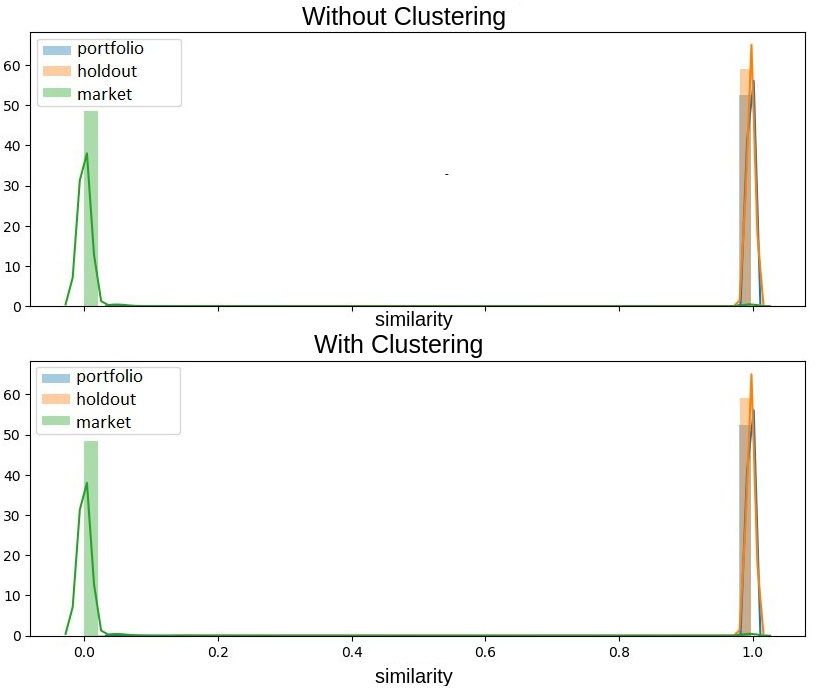
\includegraphics[width=8cm]{fig/ch4-study-4-comparsion-exp-i.png}
   \caption{Similarity distribution plot for Study 4 in experiment \nameExperimentI{}.}
   \label{fig:study-4-comparsion-exp-i}

   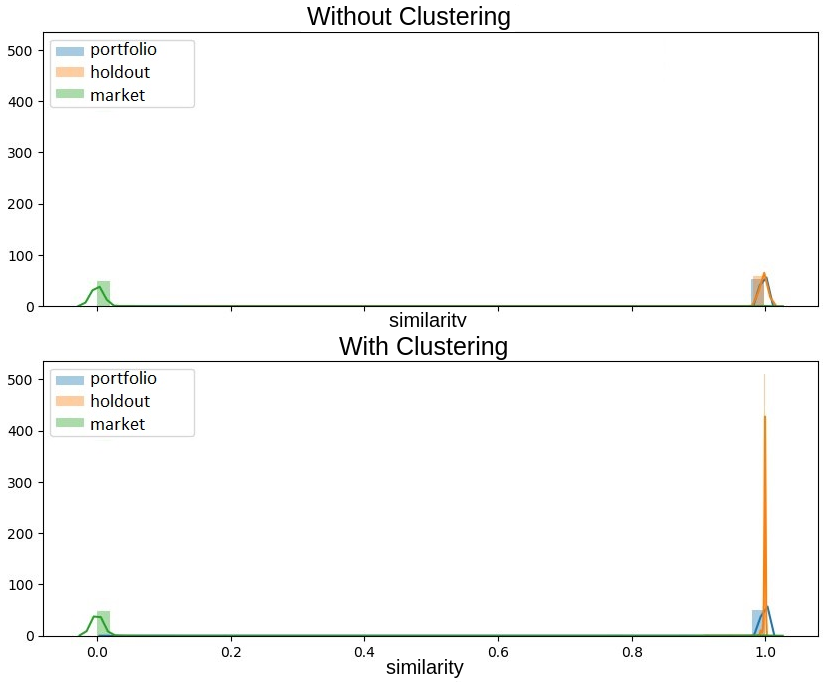
\includegraphics[width=8cm]{fig/ch4-study-4-comparsion-exp-ii.png}
   \caption{Similarity distribution plot for Study 4 for experiment \nameExperimentII{}.}
   \label{fig:study-4-comparsion-exp-ii}
\end{figure}

We can see that in experiment \nameExperimentI{} (\ref{fig:study-4-comparsion-exp-i}) the similarity distributions with and without clustering are virtually the same. This is better understood when you look at the number of clusters in its portfolio. Figure \ref{fig:study-4-pca-plot} shows its PCA plot. There is only a single cluster on the portfolio, consequentially, the result of this cluster is the same regardless of using the clustering approach.

\begin{figure}[!ht]
   \centering
   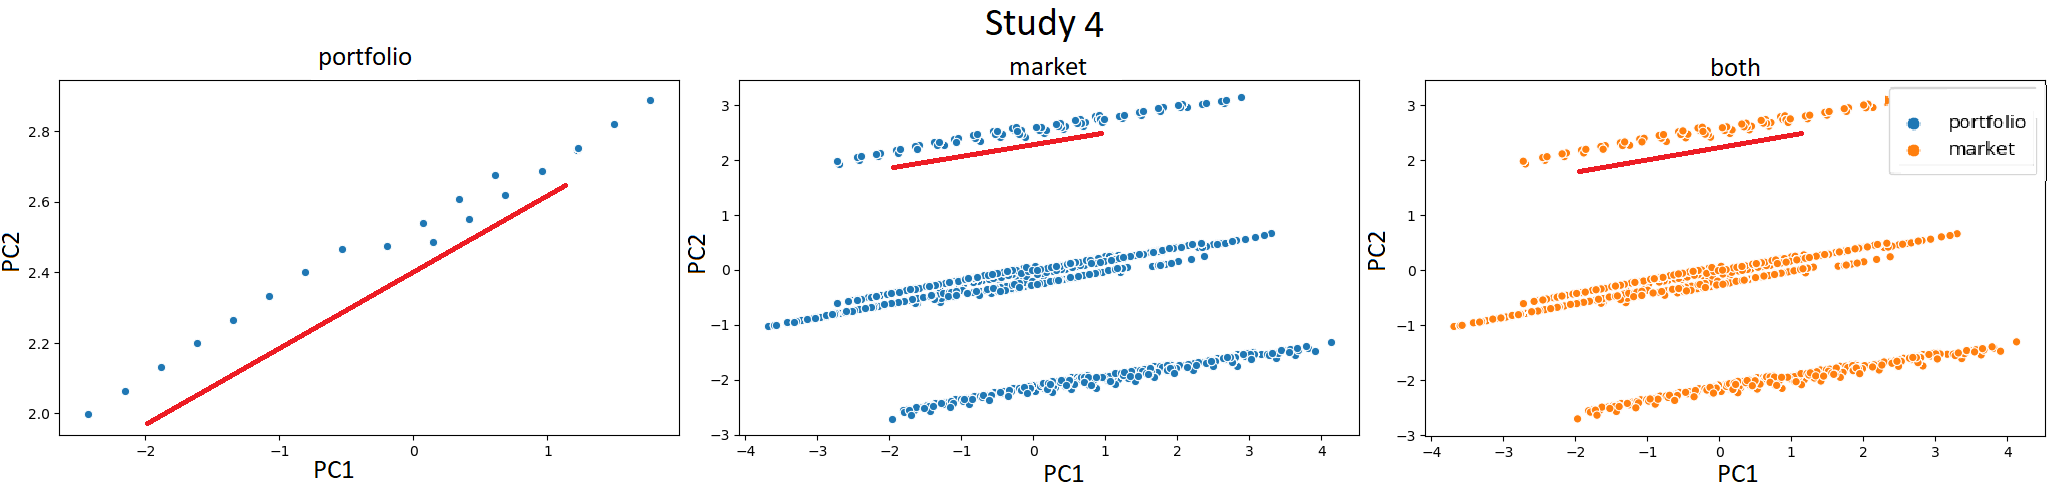
\includegraphics[width=\linewidth]{fig/ch4-study-4-pca-plot.png}
   \caption{PCA plot for Study 4. On the left there is just the portfolio, on the right both portoflio and market.}
   \label{fig:study-4-pca-plot}
\end{figure}

In \nameExperimentII{} (\ref{fig:study-4-comparsion-exp-ii}), however, there is a difference on the distributions between the with and without the clustering. Basically, the holdout set changed its distribution. In this experiment the OT scored these companies with really close scores, in other words, their standard deviation decreased. But, even though the scores of the companies (and possibly the ordering) of the holdout set changed, the lift kept the same because of how it is calculated. The same number of companies (of the holdout set) on the first decile occurred in the run without the clustering and in with the clustering, thus the value of the lift is the same for both runs.

Another study that had a zero lift gain was Study 22, in the \nameExperimentI{} experiment. Figure \ref{fig:study-22-clusters-simi-plot} shows the similarity distribution plots for the clusters' runs of this study.

Although this study has three clusters in the portfolio, only Cluster 1 has the minimum data to a valid run. Cluster 0 and Cluster 2 did not have companies on the Market, so the sixteen companies of the former and thirteen companies of the latter were discarded. Since they represent less than $0.001\%$ of the overall data of the study, the behavior is practically the same as Study 4, thus, for the same reason, the lift is the same for both runs (with and without clustering).

\begin{figure}[H]
   \centering
   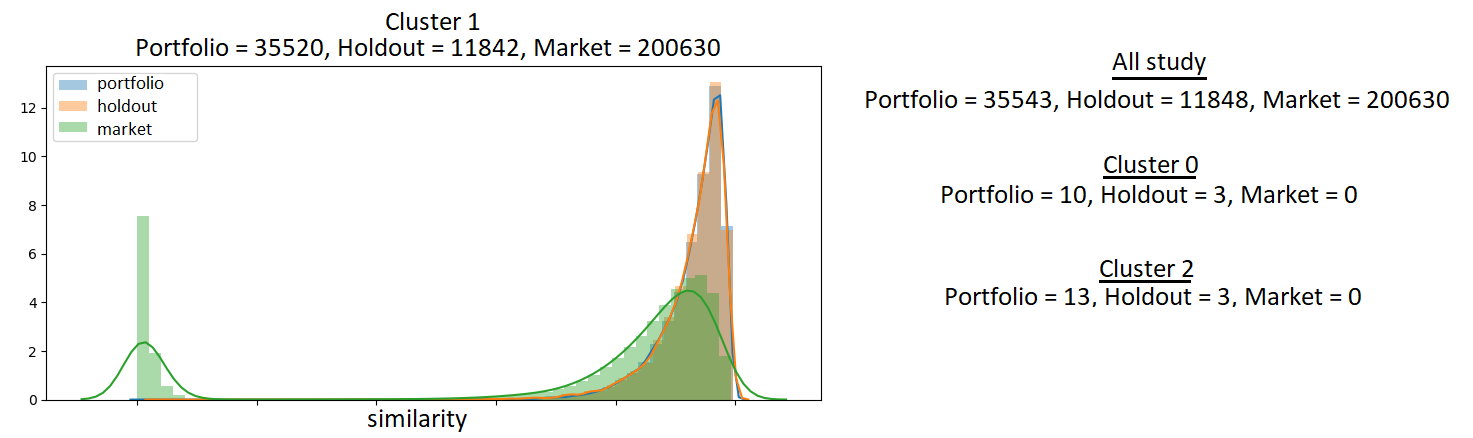
\includegraphics[width=8cm   ]{fig/ch4-study-22-clusters-simi-plot.png}
   \caption{Similarity distribution plot for the clusters' runs of Study 22 on experiment \nameExperimentI{}.}
   \label{fig:study-22-clusters-simi-plot}
\end{figure}

\subsection{Studies with marginal increase or decrease on the lift}
\label{ch:marginal-change}

Both experiments had studies that changed the lift in a minor way, positively and negatively. These studies improved or lowered the lift up to approximately $5\%$. They are presented in the light green and light red colors in both tables previously mentioned. Experiment \nameExperimentI{} had two positives and five negatives. \nameExperimentII{} had seven and five, respectively.

All of these studies had the same prevalent behavior: the overall distributions of the three sets (portfolio, holdout, and market) before and after the clustering were almost the same. There is a small difference to the holdout distribution. Figures \ref{fig:study-5-marginal-increase-exp-2} and \ref{fig:study-12-marginal-decrease-exp-1} illustrate, respectively, examples of a small increase and decrease on the lift. In the former, the similarity distributions plot for Study 5 in experiment \nameExperimentII{}, and in the latter the same plot for Study 12 for experiment \nameExperimentI{}.

\begin{figure}[!ht]
   \centering
   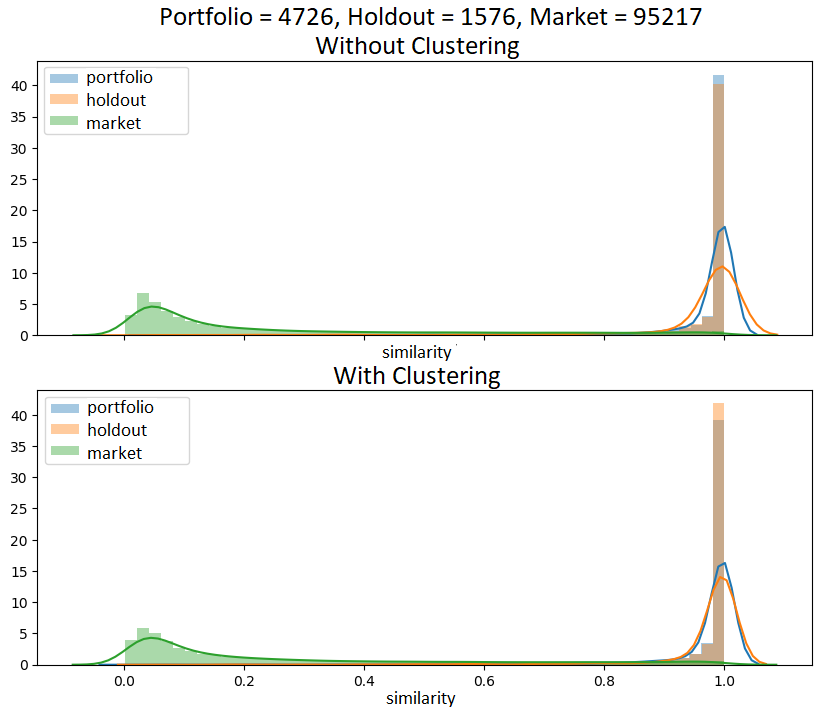
\includegraphics[width=8cm]{fig/ch4-study-5-marginal-increase-exp-2.png}
   \caption{Similarity distribution plot for Study 5 on experiment \nameExperimentII{}. An example of marginal increase on the lift.}
   \label{fig:study-5-marginal-increase-exp-2}

   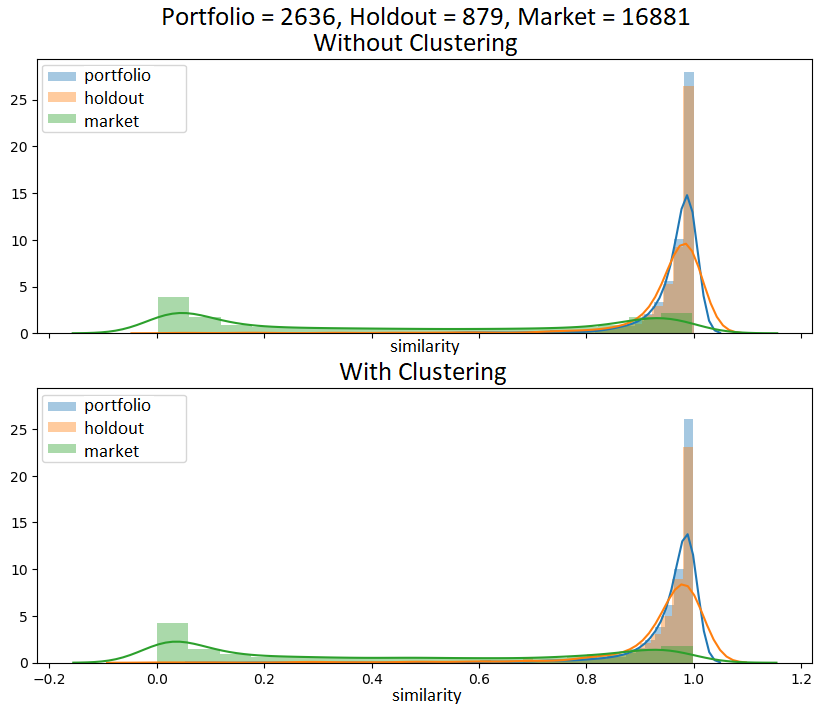
\includegraphics[width=8cm]{fig/ch4-study-12-marginal-decrease-exp-1.png}
   \caption{Similarity distribution plot for Study 12 on experiment \nameExperimentI{}. An example of marginal decrease on the lift.}
   \label{fig:study-12-marginal-decrease-exp-1}
\end{figure}

We can notice that the peak near similarity $1.0$ of the holdout set goes from approximately $37.0$ to beyond $40.0$ in Figure \ref{fig:study-5-marginal-increase-exp-2}. The opposite happens in Figure \ref{fig:study-12-marginal-decrease-exp-1}, the peak goes from almost $25.0$ to $20.0$.

\subsection{Studies with considerable increase or decrease to the lift}
\label{ch:considerable-change}

Most of the studies on both experiments had more than $5\%$ variation to the lift (positive and negative). In \nameExperimentI{}, fourteen of them were negative and only Study 2 was positive. However, in experiment \nameExperimentII{}, five were positive and four were negative.

The behavior of the similarity distributions with the clustering follows the same idea as section \ref{ch:marginal-change}, but with more exacerbate results. Figure \ref{fig:study-8-considerable-increase-exp-2} shows the similarity distributions with and without clustering for Study 8 in experiment \nameExperimentII{}, which is an example of a considerable increase on lift. In contrast, Figure \ref{fig:study-9-considerable-decrease-exp-1} displays the same plot for Study 9 in experiment \nameExperimentI{}, an example of considerable decrease on the lift.

\begin{figure}[!ht]
   \centering
   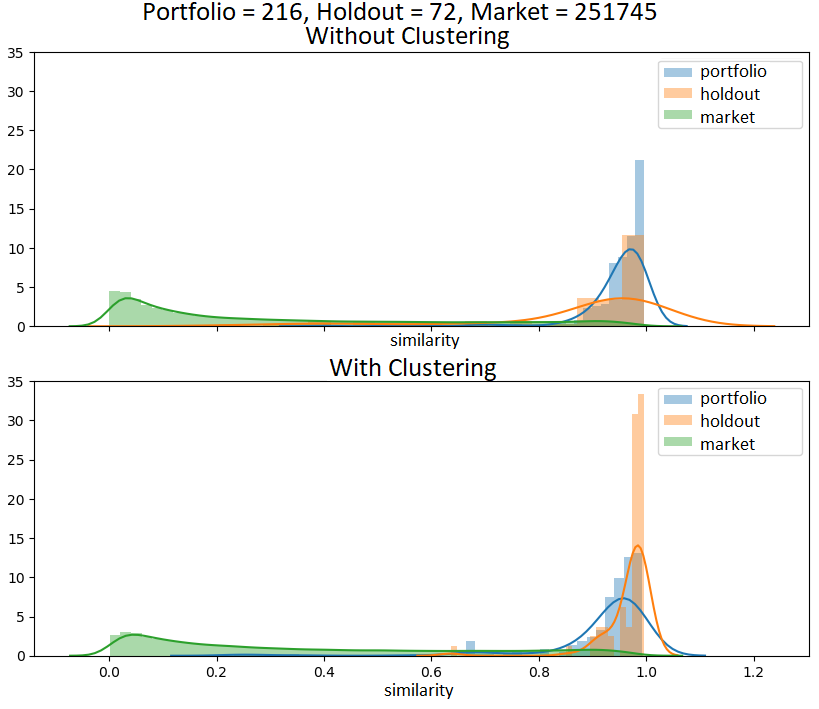
\includegraphics[width=8cm]{fig/ch4-study-8-considerable-increase-exp-2.png}
   \caption{Similarity distribution plot for Study 8 on experiment \nameExperimentII{}. An example of considerable increase on the lift.}
   \label{fig:study-8-considerable-increase-exp-2}
\end{figure}

\begin{figure}[!ht]
   \centering
   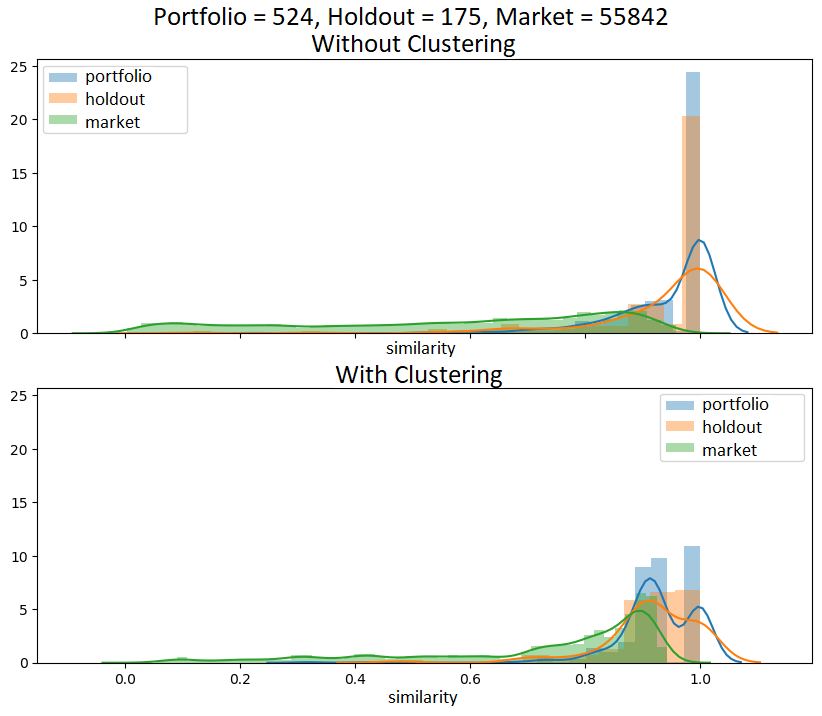
\includegraphics[width=8cm]{fig/ch4-study-9-considerable-decrease-exp-1.png}
   \caption{Similarity distribution plot for Study 9 on experiment \nameExperimentI{}. An example of considerable decrease on the lift.}
   \label{fig:study-9-considerable-decrease-exp-1}
\end{figure}

Now the difference between the distributions, in these cases, is easier to spot. In Figure \ref{fig:study-8-considerable-increase-exp-2} we can see that the peak of the holdout set rose from $10.0$ to more than $30.0$. Consequentially, the curve became more thin, meaning that its variance decreased. The contrary to this, is showed on Figure \ref{fig:study-9-considerable-decrease-exp-1}. The peak of the holdout set distribution went from $20.0$ to less than $10.0$. Also, the portfolio distribution changed. Its single peak decreased by $15$ units, and it was splitted in two peaks, one near $0.9$ similarity and the other near similarity $1.0$. Moreover, the distribution of the market skewed to the right on this run, creating a high density area near $0.9$ similarity. 

\subsection{Outliers studies}
\label{ch:outliers}

Study 24 was clearly the outlier of all studies. It got more than $200\%$ increase on the lift in both experiments. In experiment \nameExperimentII{} more three studies were considered outliers due to the interquartile range rule - the lower and upper bound in this experiment were $-14.77\%$ and $18.62\%$, respectively. These studies had similar shift on the distributions as the ones seen in \ref{ch:considerable-change}. Hence, just Study 24 is presented here. Figure \ref{fig:outlier-study-24-exp-2} exhibits the similarity distribution plot of this study in \nameExperimentII{}, and Figure \ref{fig:outlier-study-24-lift-exp-2} its lift plots, which contains the lifts of all deciles of the runs with and without the clustering.

\begin{figure}[!ht]
   \centering
   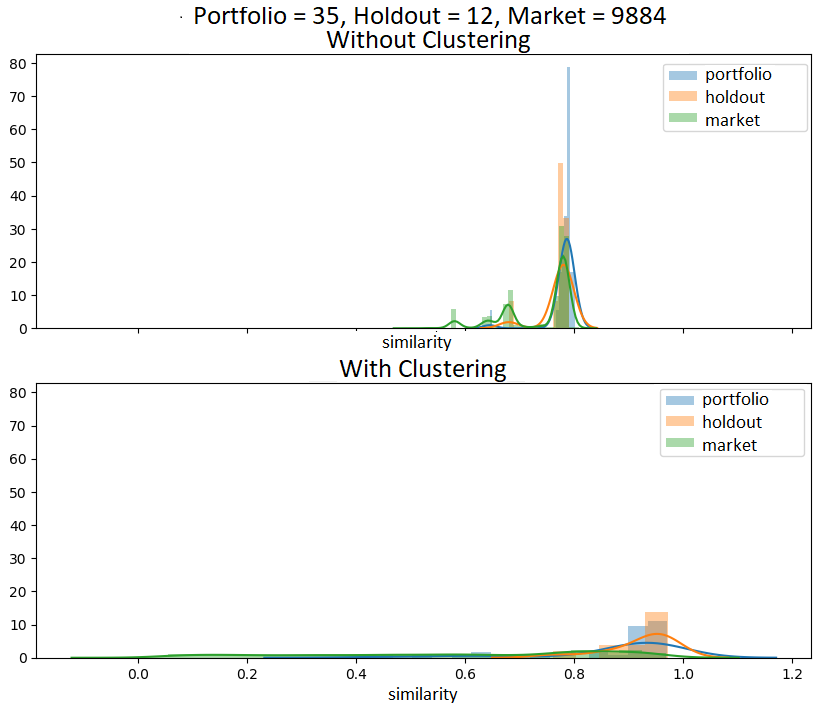
\includegraphics[width=8cm]{fig/ch4-outlier-study-24-exp-2.png}
   \caption{Similarity distribution plot for Study 24 on experiment \nameExperimentII{}.}
   \label{fig:outlier-study-24-exp-2}
\end{figure}

The main aspect of this study is presented in Figure \ref{fig:outlier-study-24-exp-2}. The Figure shows unusual distributions with multiple modes (without clustering), the highest one located at similarity $0.8$. The OT failed to classify the portfolio of this study close similarity $1.0$. Moreover, the number of companies for each of the sets of the study is unbalanced. There are only 35 companies in the portfolio and twelve in the holdout set against a market with two orders of magnitude higher. This discrepancy can be one of the issues that led this study to have odd similarity distributions.

\begin{figure}[!ht]
   \centering
   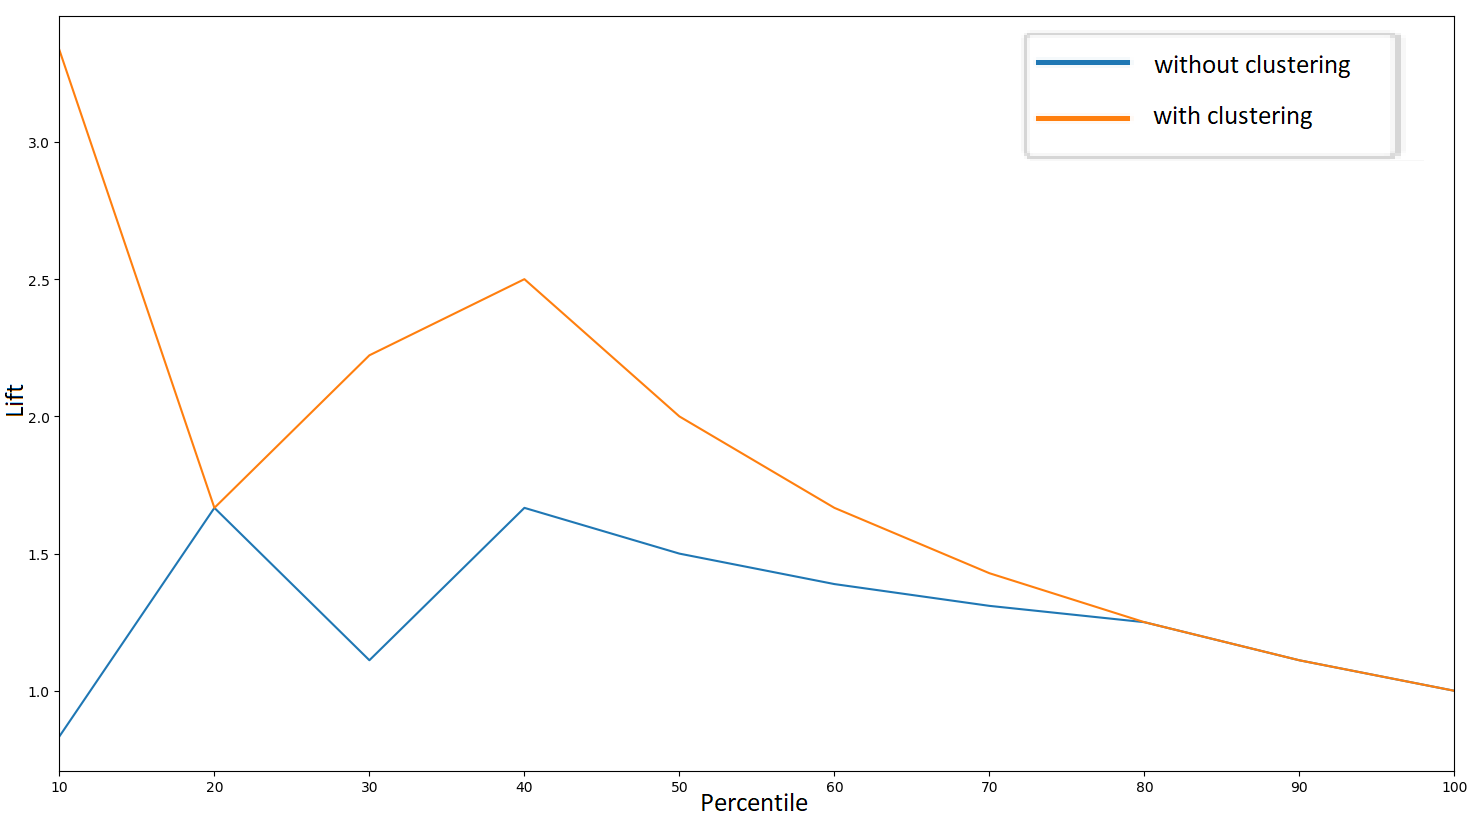
\includegraphics[width=8cm]{fig/ch4-outlier-study-24-lift-exp-2.png}
   \caption{Lift plot for Study 24 on experiment \nameExperimentII{}.}
   \label{fig:outlier-study-24-lift-exp-2}
\end{figure}

This issue is reinforced when we look at Figure \ref{fig:outlier-study-24-lift-exp-2}. The expected shape of a lift curve is in the form of a decreasing exponential, in other words, the lift of the decile on the left is greater than the one in the right, but this is not what happens on both runs of the experiment for this study. In the run with the clustering, the lift of the second decile is lower than the fourth one. On top of that, the lift of the first decile in the run without the clustering is lower than $1.0$. 

With the clustering, the distributions skewed to the right, with the holdout set being the closest to similarity $1.0$. This explains why the lift of the first decile increased over $200\%$ in the run with the clustering.

\subsection{Studies that had multiple profiles in its portfolio}

The last group of studies to be analyzed are the bolded ones in both tables (\ref{table:lift_gain_exp-i} and \ref{table:lift_gain_exp-ii}). These are the studies that sparked the idea of clustering the portfolio before running the OT. However, most of them did not had the expected behavior. Let us use one example that illustrate this result. Figure \ref{fig:bump-study-25} displays the similarity distributions plots for Study 25 for the runs in experiment \nameExperimentII{}. 

\begin{figure}[H]
   \centering
   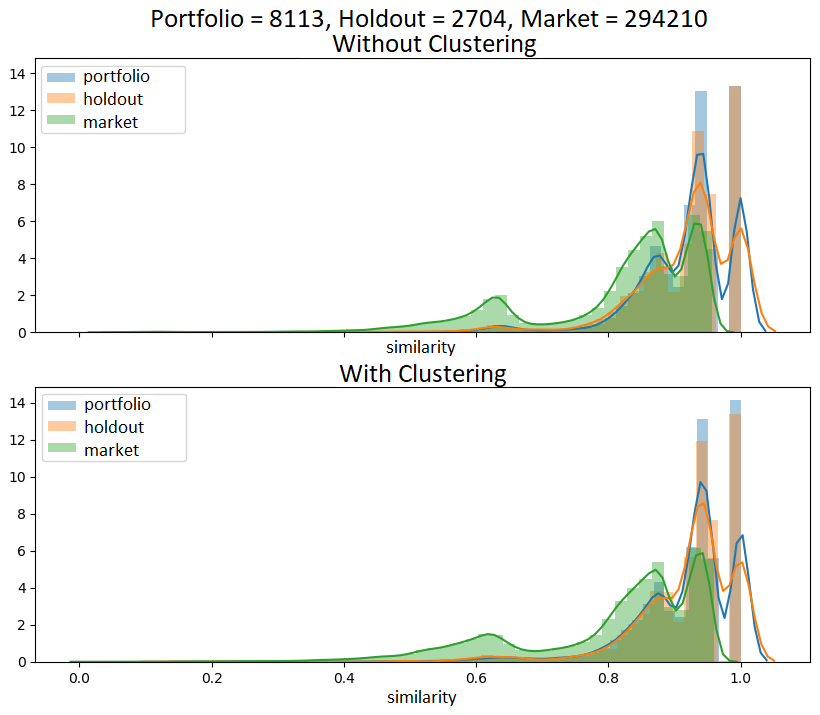
\includegraphics[width=8cm]{fig/ch4-bump-study-25.png}
   \caption{Similarity distribution plot for Study 25 on experiment \nameExperimentII{}. An example of study with multiple high density areas in the portfolio.}
   \label{fig:bump-study-25}
\end{figure}

Study 25 is a study with a positive lift gain, that is, the performance of the study improved. However, looking at Figure \ref{fig:bump-study-25} we notice that the three modes of the portfolio distributions in the run without the clustering are preserved in the run with the clustering. We expected that each one of these peaks would shift to the right, close to similarity $1.0$. 

If we take a look at each clusters' similarity distributions plot we can see more clues for this behavior. Figure \ref{fig:study-25-clusters-simi-plot} shows these plots along with the clusters' sets sizes of the runs that did not had enough data. Figure \ref{fig:study-25-pca} shows its PCA plot with the portfolio and the market. 

\begin{figure}[!ht]
   \centering
   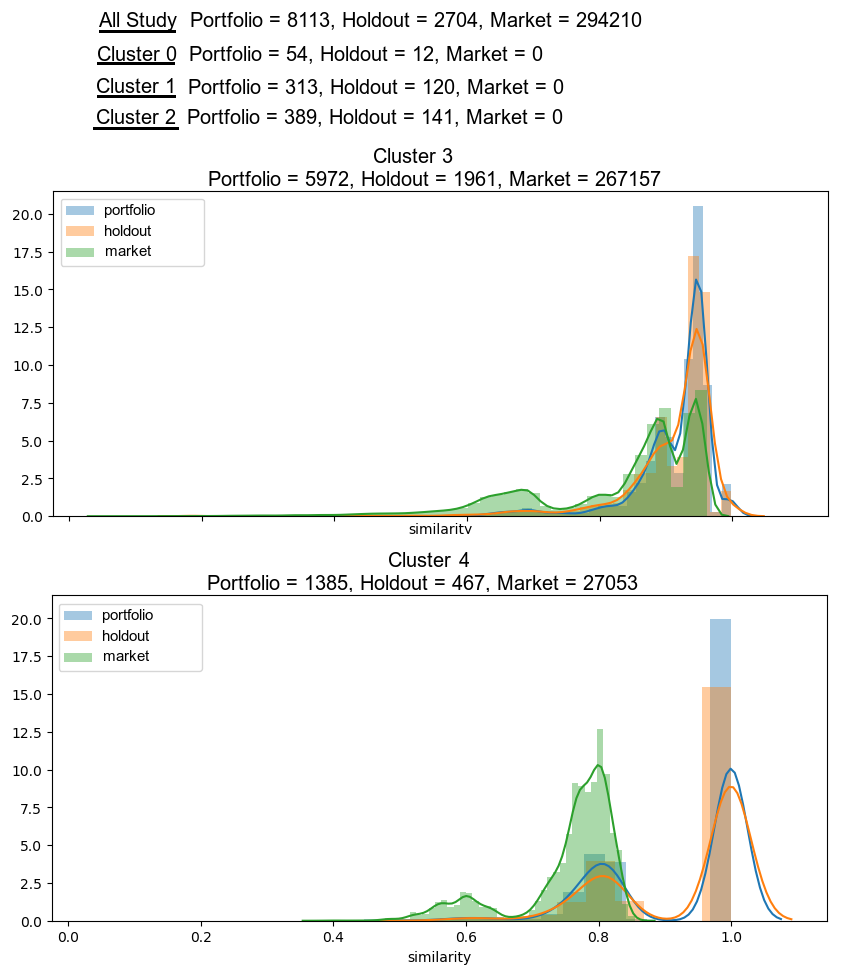
\includegraphics[width=8cm]{fig/ch4-study-25-clusters-simi-plot.png}
   \caption{Clusters' similarity distributions plots for Study 25 in experiment \nameExperimentI{}.}
   \label{fig:study-25-clusters-simi-plot}
\end{figure}

There are five cluster in the portfolio, but only two (Cluster 3 and 4) had a matching pair with the market. In these cases we see that they did not present a "one peak area" in the portfolio. Cluster 4 has two peaks: one near similarity $1.0$ and the other near $0.8$, and Cluster 3 two close peaks near similarity $0.9$. The other clusters with not enough data (0, 1, 2), the portfolio and holdout sets correspond to approximately $10\%$ of the study portfolio size. This is a small portion of the data and it only affects \nameExperimentI{}, after all, in \nameExperimentII{} there is no cluster pairing, since this information is used as a feature.

\begin{figure}[!ht]
   \centering
   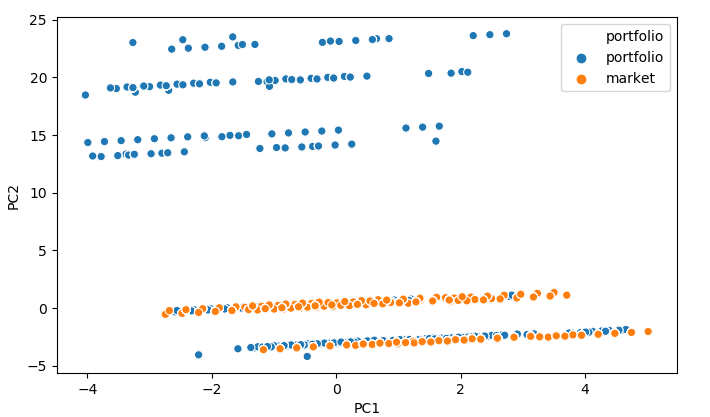
\includegraphics[width=8cm]{fig/ch4-study-25-pca.png}
   \caption{PCA plot with portfolio and market data for Study 25.}
   \label{fig:study-25-pca}
\end{figure}

The outcome of these studies demonstrate that, perhaps, \textbf{our initial hypothesis is not on point}. There still other analysis to be done, such as, analyzing the companies from the similarity perspective, for instance, seeing what the companies in the high density area near similarity $0.9$ of some study have in common. These new perspectives emerged as the work was being developed. However, because of the time constraint, they could not be prioritized in this proof of concept. 

\subsection{Other relevant studies}
\label{ch:worth-ment}

There is another study that is not in one of the specifics lift-gain groups aforementioned, but its analysis of the similarity distribution is worth to be considered. Figure \ref{fig:worth-mentioning-study-7} shows the similarity distribution plots for Study 7 in the experiment \nameExperimentII{}. 

\begin{figure}[!ht]
   \centering
   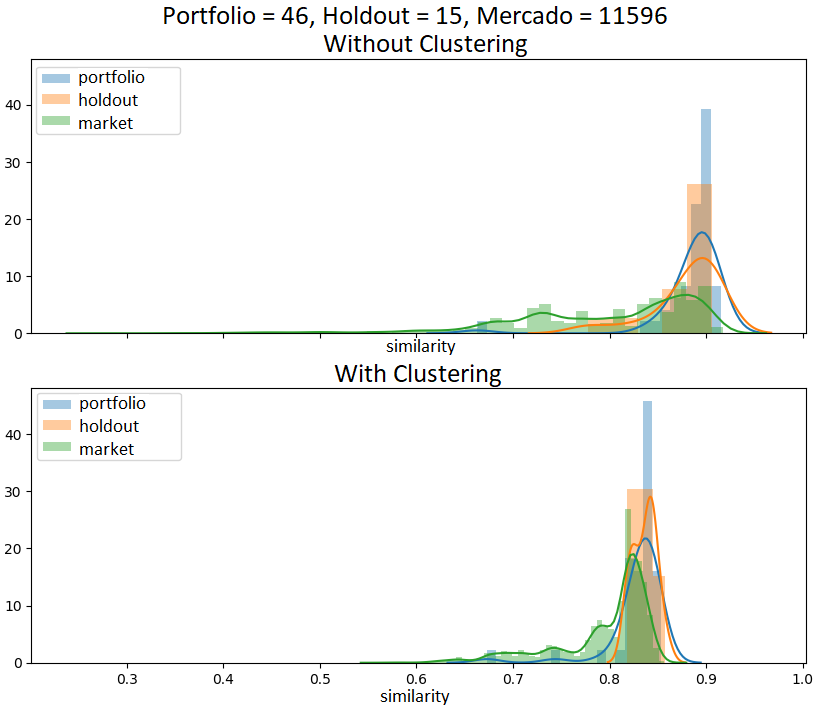
\includegraphics[width=8cm]{fig/ch4-worth-mentioning-study-7.png}
   \caption{Similarity distribution plot for Study 7 on experiment \nameExperimentII{}. Lift increased but the curves skewed to the left.}
   \label{fig:worth-mentioning-study-7}
\end{figure}

This study had a lift gain of $12.5\%$, so its performance improved, thus the expected impact in the distributions is the holdout set increase its peak near similarity $1.0$ or to shift to this region when the distribution is located more on the left of the axis. Nonetheless, the opposite happens in this study. In Figure \ref{fig:worth-mentioning-study-7}, we see that the distributions keep its shape but shifted from similarity $1.0$ to around $0.85$. But since the holdout distribution stayed more in the right, in the first decile there are more companies from the holdout set, hence the increase on the lift

The cause of this shift was not investigated. But the main point of mentioning this study is to raise the awareness of the OT's team in the choice of metrics. This example indicate that only the lift is not enough to verify the output of the OT. As seen throughout section \ref{ch:simi-distis}, the lift and the similarity distribution plot are correlated, specially the distribution of the holdout set. The lift is a metric of \underline{performance} and the similarity distribution plot shows the \underline{consistency} of the study. The shift of Study 7 was not critical, but if the similarity that the distributions went was $0.3$ instead of the $0.85$, the recommendations would not make sense for the OT's user due to its lack of consistency. That is why a new metric, that take into account consistency and performance, should be included in the overall benchmark of the studies.


\section{Experiment \nameExperimentII{} with other clustering algorithms}
\label{ch:other-clustering-algos}

The poor performance of the studies in experiment \nameExperimentI{}, which as the mean lift gain of $-9.871\%$, made the team of the OT to not proceed the testing of the clustering with this experiment. Although \nameExperimentII{} had a positive mean lift gain of $+2.016\%$, it was conducted with the "manual clustering". Thus, it was determined to oversee the results of this experiment with the other clustering algorithms previously presented in Figure \ref{fig:cluster-algo}. Figure \ref{fig:other-cluster-algo} shows the histogram of the lift gains of the re-runs for \nameExperimentII{} with KMeans (\ref{fig:other-cluster-algo:kmeans}), Gaussian Mixture (\ref{fig:other-cluster-algo:gmm}), and Bayesian Gaussian Mixture (\ref{fig:other-cluster-algo:bgm}).

\begin{figure}[!ht]
    \begin{subfigure}{.5\linewidth}
        \centering
        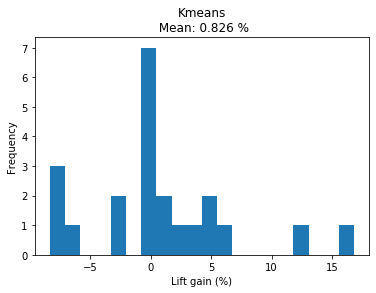
\includegraphics[width=5.5cm]{fig/ch4-kmeans_lift_gain_hist.png}
        \caption{}
        \label{fig:other-cluster-algo:kmeans}
    \end{subfigure}
    \begin{subfigure}{.5\linewidth}
        \centering
        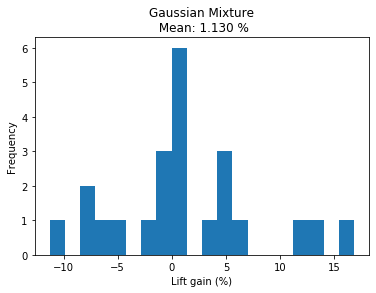
\includegraphics[width=5.5cm]{fig/ch4-gmm_lift_gain_hist.png}
        \caption{}
        \label{fig:other-cluster-algo:gmm}
    \end{subfigure}\\[1ex]
    \begin{subfigure}{\linewidth}
        \centering
        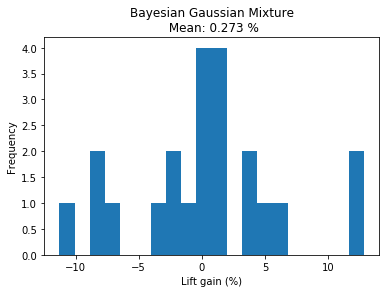
\includegraphics[width=5.5cm]{fig/ch4-bgm_lift_gain_hist.png}
        \caption{}
        \label{fig:other-cluster-algo:bgm}
    \end{subfigure}
    \caption{Lift gain histogram without outliers of other clustering algorithm runs for experiment \nameExperimentII{}}
    \label{fig:other-cluster-algo}
\end{figure}

We notice that none of them reached the lift gain of the "manual clustering". The closest one was the Gaussian Mixture with $1.13\%$. The other two resided below $1\%$ ($0.8$ for KMeans and approximately $0.3$ for Bayesian Gaussian Mixture). The outcome of these results consolidate the strategy of cluster the studies manually, meaning that the groups in the PCA plots make sense, at least in the performance perspective of the OT. 

Despite of this confirmation on the strategy adopted by the team, this is not feasible for the OT, since it is impossible to the system run in production with human interference during the leads scoring. The clustering done manually could be use as a success criteria for other clustering algorithms, but that would turn the type of problem to a classification, due to the presence of the labels.

Another alternative to improve the performance in experiment \nameExperimentII{} without the manual clustering, is to tweak the hyper-parameters of the Gaussian Mixture and see if it the lift gain approaches the achieved mark of $2\%$. For instance, in the Scikit-learn Python package, this algorithm has up to seven different hyper parameters that go from initialization, weights settings up to convergence settings \cite{scikit-learn}.
  \chapter{Conclusion} \label{cha:conclusion}

In this work we showed how awesome this is

\section*{Future work}

 Lorem ipsum dolor sit amet, consectetur adipiscing elit. Phasellus sodales justo et fringilla ultricies. Proin sollicitudin, dolor sit amet commodo iaculis, justo mi hendrerit arcu, quis eleifend diam felis lobortis nulla. Integer aliquam quam vel nulla bibendum rutrum. Proin nec est velit. Nullam ac porta dolor. Phasellus facilisis tincidunt sem, eget ullamcorper quam imperdiet in. Quisque efficitur dictum dolor et commodo. 
 
\begin{enumerate}
  \item next point to be worked on 
  \item next point to be worked on 
  \item next point to be worked on 
  \item next point to be worked on 
  \item next point to be worked on 
\end{enumerate}

  \renewcommand{\bibname}{Bibliography}
\bibliographystyle{unsrt} % Exibir em ordem de citação
%\bibliographystyle{plain} % Exibir em ordem alfabética
\bibliography{content/references.bib} 


  \appendix
  \label{pg:arabic-count}
  \cleardoublepage
\end{document}
